%%
%% This is file `mcmthesis-demo.tex',
%% generated with the docstrip utility.
%%
%% The original source files were:
%%
%% mcmthesis.dtx  (with options: `demo')
%%
%% -----------------------------------
%%
%% This is a generated file.
%%
%% Copyright (C)
%%       2010 -- 2015 by Zhaoli Wang
%%       2014 -- 2019 by Liam Huang
%%       2019 -- present by latexstudio.net
%%
%% This work may be distributed and/or modified under the
%% conditions of the LaTeX Project Public License, either version 1.3
%% of this license or (at your option) any later version.
%% The latest version of this license is in
%%   http://www.latex-project.org/lppl.txt
%% and version 1.3 or later is part of all distributions of LaTeX
%% version 2005/12/01 or later.
%%
%% This work has the LPPL maintenance status `maintained'.
%%
%% The Current Maintainer of this work is Liam Huang.
%%
%%
%% This is file `mcmthesis-demo.tex',
%% generated with the docstrip utility.
%%
%% The original source files were:
%%
%% mcmthesis.dtx  (with options: `demo')
%%
%% -----------------------------------
%%
%% This is a generated file.
%%
%% Copyright (C)
%%       2010 -- 2015 by Zhaoli Wang
%%       2014 -- 2019 by Liam Huang
%%       2019 -- present by latexstudio.net
%%
%% This work may be distributed and/or modified under the
%% conditions of the LaTeX Project Public License, either version 1.3
%% of this license or (at your option) any later version.
%% The latest version of this license is in
%%   http://www.latex-project.org/lppl.txt
%% and version 1.3 or later is part of all distributions of LaTeX
%% version 2005/12/01 or later.
%%
%% This work has the LPPL maintenance status `maintained'.
%%
%% The Current Maintainer of this work is Liam Huang.
%%
\documentclass{mcmthesis}
\mcmsetup{CTeX = true,    % 使用 CTeX 套装时，设置为 true
          tcn = {2616003}, problem = \textcolor{red}{A},
          sheet = true, titleinsheet = true, keywordsinsheet = true,
          titlepage = false, abstract = false}
\usepackage{newtxtext}     % \usepackage{palatino}
\usepackage[numbers]{natbib}
\usepackage{tocloft}
\usepackage{tabularx}
\usepackage{makecell}
\usepackage{float}
\usepackage{subcaption}
\usepackage{graphicx}
\usepackage{gensymb}
\usepackage{xcolor}
\usepackage{soul}
\usepackage{hyperref}
\usepackage{etoolbox}
\hypersetup{
  colorlinks=true,
  linkcolor=blue,   % 正文交叉引用（\ref, \autoref）为蓝色
  citecolor=red,
  urlcolor=black
}
\usepackage{algorithm}
\usepackage{algorithmic}
\usepackage{rotating} % 导言区
\usepackage{tikz}
\usetikzlibrary{arrows.meta, positioning, shapes.geometric}
\newcommand{\Rmnum}[1]{\uppercase\expandafter{\romannumeral #1}}  %定义命令输入大写罗马数字
\newcommand{\rmnum}[1]{\romannumeral #1}  %定义命令输入小写罗马数字

% Force English abstract heading even when ctex is loaded.
%\ctexset{abstractname = {Summary}}
\renewcommand{\abstractname}{Summary}

\sethlcolor{yellow!40}
\newcommand{\hltext}[1]{\colorbox{yellow!40}{#1}}
\setlength{\cftbeforesecskip}{6pt}
\renewcommand{\contentsname}{\hspace*{\fill}\Large\bfseries Contents \hspace*{\fill}}

\title{When the Icon Turns Red: Unveiling the Hidden Dynamics Behind Battery }
% \author{\small \href{http://www.latexstudio.net/}
%   {
\includegraphics[width=7cm]{mcmthesis-logo}}}
\date{\today}
\begin{document}
\begin{abstract}
Smartphone battery endurance remains notoriously unpredictable due to coupled thermal-load dynamics.
This paper develops a continuous-time multi-physics framework for accurate \textbf{State-of-Charge (SOC) estimation and Time-to-Empty (TTE) prediction}.

\textbf{Firstly}, based on the second-order RC equivalent circuit model, we employed \textbf{the Genetic Algorithm (GA)} to conduct global optimization identification of the key parameters of the battery.
We also used the $100mA$ constant current discharge experimental data to validate the model.
\textbf{The results show} that the Genetic Algorithm can effectively identify the equivalent parameters of the mobile phone battery,
ensuring a good consistency between the output voltage of the model and the measured voltage, with an average error rate within 0.5\%.
On this basis, we introduced \textbf{the power load model and the thermodynamic model},
coupled modeling the electro-thermal behavior of the battery,
and constructed a continuous-time lithium-ion battery model applicable to dynamic load conditions. 

\textbf{Subsequently}, based on the aforementioned model, \textbf{the Unscented Kalman Filter (UKF)} method was employed to establish the TTF prediction model, enabling dynamic predictions of the remaining usage time and service life of the battery under different usage scenarios and different initial SOC conditions. 
The experimental settings covered four typical usage scenarios: \textbf{Standby, Video, Navigation, and Game}, as well as 16 combinations of initial SOC  ranging from 100\% to 20\%.
The results demonstrated that the model exhibited excellent prediction accuracy under all test conditions,
\textbf{with the average $3\sigma$ prediction error controlled within the range of 2.66\%–8.50\%}.
This verified the effectiveness and robustness of the method in complex dynamic scenarios. 

\textbf{Then}, by systematically adjusting key parameters such as \textbf{environmental temperature, screen brightness, and network data traffic, as well as related assumptions},
we conducted a model sensitivity analysis.
\textbf{The analysis results} showed that the impact of environmental temperature on battery life mainly manifested in low-load standby scenarios,
where the battery life decreased by approximately 7\% under low-temperature conditions;
while in medium-high load scenarios such as video, navigation, and gaming, its impact could be largely ignored.
\textbf{At the same time}, compared to short-term battery performance, screen brightness and network throughput are more sensitive to \textbf{the long-term lifespan of the battery}. 
Reducing screen brightness and network data load can significantly delay the battery aging process. 

\textbf{Ultimately}, building on our findings, we recommend targeted \textbf{strategies for end-users and OS developers} to enhance battery longevity.
 Users should mitigate sustained high-load usage and moderate screen brightness and network activity. For OS designers, we advocate integrating thermal-aware CPU throttling and dynamic power management to prolong overall device lifespan.

 \begin{keywords}
SOC estimation \quad Remaining time prediction \quad Genetic algorithm \quad Univariate Kalman filtering \quad Smart phone \quad Lithium battery
\end{keywords}
\end{abstract}

\maketitle

%% Generate the Table of Contents, if it's needed.
% \renewcommand{\contentsname}{\centering Contents}.
\pretocmd{\tableofcontents}{%
  \hypersetup{linkcolor=black}%
}{}{}
\apptocmd{\tableofcontents}{%
  \hypersetup{linkcolor=blue}%
}{}{}

\tableofcontents        % 若不想要目录, 注释掉该句
\thispagestyle{fancy}


\newpage









\section{Introduction}
\subsection{background}
With the development of science and technology, mobile phones play an indispensable role in our lives.
By 2025, the number of global mobile phone users had exceeded 7.3 billion.The battery life of the phone directly affects the user experience. 
As the core component of the phone, the battery works together with the screen, CPU operation, network load, and applications to determine the phone's battery life.
\begin{figure}[H]
  \centering
  \begin{subfigure}[b]{0.48\textwidth}
    \centering
    
\includegraphics[width=\linewidth]{figures/image.png}
    \caption{Global number of mobile phone users\cite{statista_smartphone_2025}}
  \end{subfigure}\hfill
  \begin{subfigure}[b]{0.48\textwidth}
    \centering
    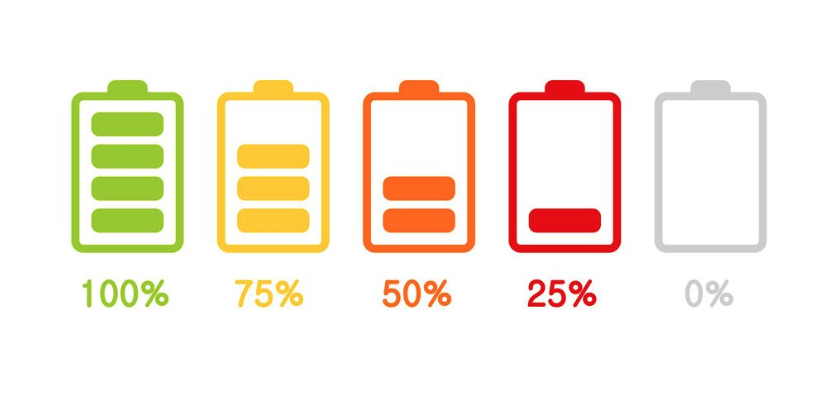
\includegraphics[width=\linewidth]{figures/R-C.png}
    \caption{Schematic diagram of mobile phone battery capacity}
  \end{subfigure}
  \caption{}
  \label{fig:battery_parallel}
\end{figure}
\vspace{-0.4cm}
\subsection{Restatement of the Problem}
Based on the above understanding, our task is to establish a time-domain model to describe the evolution of the State of Charge (SOC) over time in practical usage scenarios. Specifically, this study will attempt to accomplish the following tasks:
\begin{itemize}
  \item \textbf{Task 1:} Establish a continuous-time model to represent the battery's charge state, and the model can extend from simple battery discharge states to complex multi-scenario conditions.
  \item \textbf{Task 2:} Use the above model to predict battery performance under different initial charge levels and usage scenarios.
                        Analyze the results to quantify the model's uncertainty and effectiveness. 
  \item \textbf{Task 3:} Conduct sensitivity analysis on the established model by adjusting assumptions and model parameters.
  \item \textbf{Task 4:} Develop corresponding suggestions for end users and operating system designers to enhance the battery life.
\end{itemize}
\subsection{Literature Review}
Accurate State of Charge (SOC) estimation is a core function of advanced Battery Management Systems (BMS). In the field of electric vehicles, Hui Pang and Fengqi Zhang proposed a parameter identification framework and an SOC estimation method for lithium-ion battery equivalent circuit models based on Adaptive Extended Kalman Filtering (AEKF) \cite{en11051033}. Yixing Chen, Deqing Huang, et al. developed an improved second-order RC model incorporating fractional calculus to better capture lithium-ion battery dynamics \cite{en10091313}. These studies demonstrate that equivalent circuit models combined with advanced filtering algorithms can achieve high SOC estimation accuracy under dynamic operating conditions.

In mobile consumer electronic devices, limited battery capacity has motivated extensive research on power consumption modeling and energy management strategies \cite{aa}. Prior work has analyzed smartphone energy consumption at the system level, constructed power models focusing on high-energy components such as CPU, GPU, and display, and predicted overall device power consumption under varying workloads to estimate battery usage and remaining operating time \cite{en4040582}. Moreover, dynamic offloading techniques applied to mobile device energy models—covering CPU, display, wireless interfaces, and memory—have been shown to improve energy efficiency by 18\% to 55\%, depending on operating conditions \cite{ALI2016173}. Collectively, these studies highlight the critical influence of user behavior and system load on battery consumption and provide a theoretical and empirical foundation for parameter selection in multi-scenario battery models.\subsection{Our Work}
Inspired by the aforementioned research, the specific process of our study is shown in \autoref{fig:process}:
\begin{figure}[H]
  \centering
  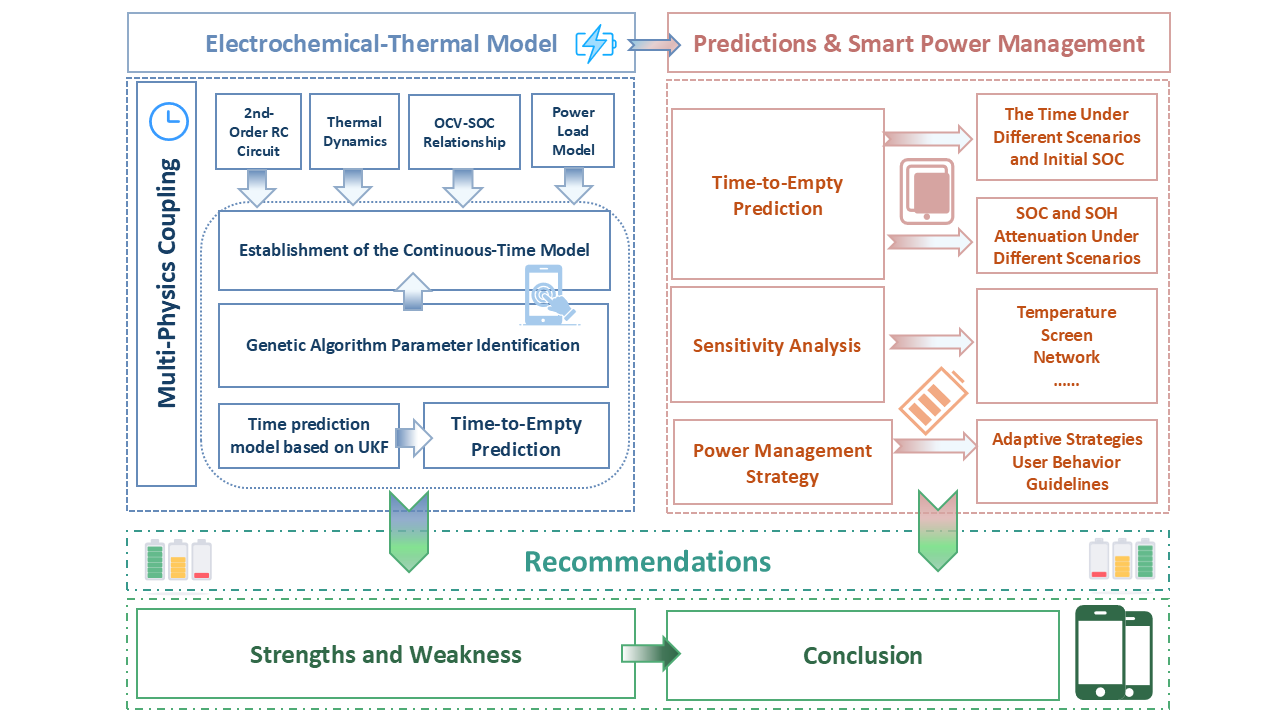
\includegraphics[width=1\textwidth]{figures/our.png}
  \caption{Flowchart}
  \label{fig:process}
\end{figure}

\section{Assumptions and Justification}
\textbf{Assumption 1:}
The mobile phone power management link exhibits approximately constant power absorption at the battery side.

Due to regulated power supply architectures, the battery-side behavior can be reasonably approximated as constant power, simplifying system coupling while maintaining physical consistency.

\textbf{Assumption 2:}
The open-circuit voltage $E(SOC)$ depends only on $SOC$ and is approximated by an offline fitted polynomial $E(z)$ within a given temperature range.

This approximation replaces lookup-table methods, avoids additional electrochemical states, and ensures tractable UKF implementation.

\textbf{Assumption 3:}
The total power $P(t)$ is decomposable into additive scenario-based components (e.g., standby, screen, CPU, GPS, network).

This enables multi-scenario modeling and sensitivity analysis beyond simple discharge conditions.

\textbf{Assumption 4:}
The battery temperature $T(t)$ is spatially uniform and follows Newton’s law of cooling over short time intervals.

A lumped thermal model captures the dominant temperature dynamics while keeping electro-thermal coupling low-dimensional.
\section{Notations}

\begin{table}[H]
\centering
\caption{Key notations used in this paper}
\vspace{-0.4cm}
\begin{tabularx}{0.92\textwidth}{lXc}
\toprule
Symbol & Description & Unit \\
\midrule
$SOC(t)$ & State of Charge  & -- \\
$U(t)$ & Battery terminal voltage & V \\
$E(SOC)$ & Open-circuit voltage (OCV)  & V \\
$i(t)$ & Battery current & A \\
% $\Delta t$ & Sampling period / discretization step & s \\
$R_0$ & Ohmic internal resistance & $\Omega$ \\
$R_1,\,R_2$ & Polarization resistances in the 2-RC model & $\Omega$ \\
$C_1,\,C_2$ & Polarization capacitances in the 2-RC model & F \\
$U_1(t),\,U_2(t)$ & RC polarization voltages & V \\
$Q_n$ & Rated/available battery capacity & Ah \\
$P(t)$ & Total phone power demand (load power) & W \\
$T(t)$ & Battery/device temperature & $^\circ$C \\
$T_{env}$ & Ambient temperature & $^\circ$C \\
$SOH(t)$ & State of Health (capacity/health indicator) & -- \\
\bottomrule
\end{tabularx}
\end{table}
\section{The Continuous-Time Model }
\subsection{Establishment of The Model}
\subsubsection{Model \Rmnum{1}: Battery Equivalent Circuit Model}
The problem statement explicitly assumes the smartphone battery is a lithium battery.
Considering various polarization effects during lithium battery charge and discharge processes, including ohmic polarization, electrochemical polarization, and concentration polarization,
and balancing model computational complexity with fidelity,
we select a second-order RC equivalent circuit model to simulate the internal structure of the lithium battery, approximately describing the internal dynamic processes. Its equivalent circuit is shown in \autoref{fig:battery_model}.
\begin{figure}[htbp]
  \centering
  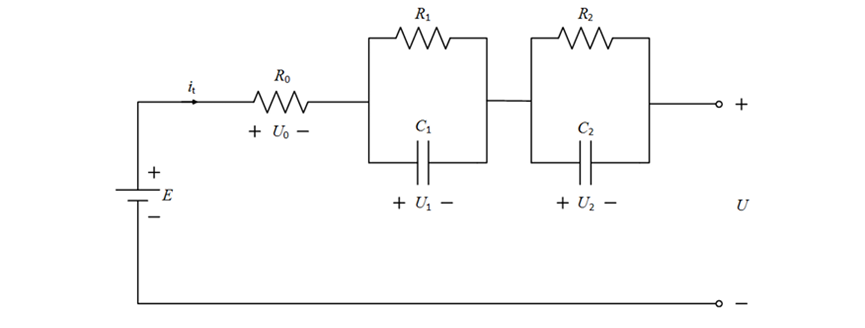
\includegraphics[width=0.8\textwidth]{figures/battery_model.png}
  \caption{Second-order RC equivalent circuit model schematic}
  \label{fig:battery_model}
\end{figure}

Where,$E$ represents the open-circuit voltage of the battery, which depends on the State of Charge (SOC) and is a function indicating the battery's state of charge (SOC).
$i_t$ is the total current in the circuit, and $U$ is the output voltage of the battery.
According to Kirchhoff's laws, the expression for the output voltage $U$ of the battery can be derived as follows: $i_t$ is the total current in the circuit, and $U$ is the output voltage of the battery.
\begin{equation}
  U=E-U_0-U_1-U_2
\end{equation}
Where the voltage drop across the ohmic resistance satisfies Ohm's law $U_0=i_t\ast R_0$, thus:
\begin{equation}
 U=E(SOC)-i_t\ast R_0-U_1-U_2   
\end{equation}
Meanwhile, according to Kirchhoff's Current Law, the current relationship in the first parallel circuit satisfies $i_t = i_{R1} + i_{C1}$,
therefore, the differential equation of the first circuit can be expressed as:
\begin{equation}
  \frac{dU_1}{dt}=\frac{i_t}{C_1}-\frac{U_1}{R_1C_1}
\end{equation}
For the second parallel circuit, by the same reasoning, we can obtain:
\begin{equation}
  \frac{dU_2}{dt}=\frac{i_t}{C_2}-\frac{U_2}{R_2C_2}
\end{equation}
To close the model for solution, we define the SOC change equation:
\begin{equation}
  \frac{dSOC}{dt}=-\frac{i_t}{Q_n}
\end{equation}
Where $Q_n$ is the battery's rated capacity, and the negative sign indicates that discharging causes SOC to decrease.
In summary, the state equations of the battery model can be obtained:
\begin{equation}
  \begin{cases}
    \dfrac{dU_1}{dt} = \dfrac{i(t)}{C_1} - \dfrac{U_1}{R_1C_1} \\[8pt]
    \dfrac{dU_2}{dt} = \dfrac{i(t)}{C_2} - \dfrac{U_2}{R_2C_2} \\[8pt]
    \dfrac{d(SOC)}{dt} = -\dfrac{i(t)}{Q_n}
  \end{cases}
\end{equation}
and the corresponding output equation:
\begin{equation}
  U(t)=E(SOC)-i(t)\ast R_0-U_1-U_2
\end{equation}
\subsubsection{Model \Rmnum{2}: Power Load Model}
 In the actual discharge process of the phone, the battery discharge current is not a constant rated value, but is determined by the instantaneous power demand of various phone components;
 At the same time, the power demand can be mapped from the user's usage behavior.
 Based on this, we decompose the total power output of the battery into base standby power $P_{base}$, screen usage power $P_{screen}$, CPU usage power $P_{CPU}$,
 GPS usage power $P_{GPS}$, network usage power $P_{networking}$, and background power $P_{background}$,
 obtaining the total power expression:
 \begin{equation}
    P(t)=P_{base}+P_{screen}(t)+P_{CPU}(t)+P_{GPS}(t)+P_{networking}(t)+P_{background}(t)
  \end{equation}
 On the other hand, the power management chip inside the phone usually draws power from the battery in an approximately constant power mode. According to the power definition $P=UI$, the battery current $i(t)$ can be expressed as:
  \begin{equation}
  i(t)=\frac{P}{U(t)\ast\eta}
  \end{equation}
  where $\eta$ is the efficiency of the DC-DC converter, usually taken as a constant close to 1. $U(t)$ is the output voltage at the battery terminal.
To accurately characterize the power characteristics of the phone under different usage scenarios, we have established mathematical models for each power-consuming component based on physical principles and measured data.
\subparagraph{Base Power Consumption}
Base power consumption $P_{{base}}$ represents the minimum power required to keep the system alive when the phone is turned on but there is no user activity, including necessary overhead such as the operating system kernel, clock chip, and memory standby. This item is a constant:
\begin{equation}
    P_{{base}} = P_0
\end{equation}
where $P_0$ is usually between 0.2-0.5 W, depending on the specific phone model.
\subparagraph{Screen Power Consumption Model}
According to Weber's law, the human eye perceives light intensity logarithmically. Therefore, to make the user perceive brightness changes linearly, the actual screen output power must increase exponentially or as a power function. We define the screen power consumption model as:
\begin{equation}
   P_{screen}(t)=\delta _{on}(t)*P_{drive}+\alpha_s*(B(t)^\gamma)
\end{equation}
where:
$\delta_{on}(t) \in \{0,1\}$ represents the screen on/off status,
$P_{drive}$ is the basic power consumption for screen driving,
$B(t) \in (0,1)$ is the screen brightness percentage,
$\gamma$ is the gamma correction coefficient, usually ranging from 1.5 to 2.2.
According to the measured data from reference \cite{Carroll2010Power},
 in practical applications, the following values are adopted:
\begin{equation}
    P_{screen}(t) = 1.08 + 0.72 \cdot B(t)^{2} 
\end{equation}
\subparagraph{Processor Power Consumption Model}
Physically, the dynamic power consumption of integrated circuits satisfies $P = C \cdot V^2 \cdot f$,
For modern CPUs, as the load $u$ increases, not only does the frequency $f$ increase, but the voltage $V$ also increases.
Since the voltage $V$ is usually proportional to the frequency $f$, the power consumption is proportional to the cube of the frequency.
And because the CPU utilization $u$ is positively correlated with the frequency $f$, the relationship between power consumption and utilization is nonlinear.
We use a quadratic polynomial to simulate this phenomenon:
\begin{equation}
    P_{CPU}(t) = P_{idle} + \beta _1 \cdot u(t) + \beta _2 \cdot u(t)^2
\end{equation}
where:
$P_{idle}$ is the CPU idle power,
$u(t) \in [0,1]$ is the CPU utilization,
$\beta _1, \beta _2$ are model coefficients.
These parameters are determined by boundary conditions,
with the CPU minimum operating power being 0.36 W (at $u=0.1$),
maximum operating power being 2.88 W (at $u=1$). 
Considering that the phone is mostly in a low-load state most of the time, the linear power consumption accounts for the major proportion. 
Therefore, we take $\beta_1=2.58$ and $\beta_2=0.2$:
\begin{equation}
    P_{CPU}(t) = 0.1 + 2.58 \cdot u(t) + 0.2 \cdot u(t)^2 
\end{equation}
\subparagraph{GPS Power Consumption Model}
GPS typically consumes the most power during the startup phase (active phase), and the power consumption significantly decreases after successful positioning. The GPS power consumption model is defined as:
\begin{equation}
P_{GPS}(t)=\delta _{gps}(t)*P_{GPS-active}
\end{equation}
where $\delta _{gps}(t)\in \{0,1\}$ represents the GPS on/off status, and $P_{GPS-active}$ is the power consumption when GPS is active.
\subparagraph{Network Power Consumption Model}
According to communication principles, to maintain a constant signal-to-noise ratio for connection, when the distance increases or obstacles increase (signal strength $S$ decreases), the phone must increase the transmission power. The model is defined as:
\begin{equation}
    P_{networking}(t) = \delta_{network}(t) \cdot (P_{base_net}+\frac{P_{ref}}{S_{signal}(t)}\ast D_{throughput}(t))
\end{equation}
where
$\delta_{network}(t) \in \{0,1\}$ represents the network module on/off status,
$S_{signal}(t)\in (0,1]$ is the signal strength factor, with 1 indicating the best signal,
$D_{throughput}(t)$ is the data transmission rate (Mbps),
$P_{ref}$ is the reference transmission power, generally taken as 0.3-0.4 W.
\subparagraph{Background Task Power Consumption Model}
The main characteristic of background tasks is intermittency; they do not run continuously but are periodically awakened. We introduce a pulse sequence model:
\begin{equation}
    P_{background}(t) = \sum_{k} P_{task} \cdot \prod (\frac{t - t_k}{\tau })
\end{equation}
where $\prod $ is the rectangular window function, indicating that the task lasts for a short period,
 $t_k$ represents the time point of the $k$-th wake-up,
 $P_{task}$ is the power during wake-up, determined by the phone's working state.
The rectangular window function is defined as:
\begin{equation}
    \prod (\frac{t - t_k}{\tau }) = \begin{cases}
        1 & t_k \leq t < t_k + \tau \\
        0 & \text{otherwise}
    \end{cases}
\end{equation}
where $\tau$ is the duration of a single background task.
\subsubsection{Model \Rmnum{3}: Thermodynamic Model}
Temperature is a key factor influencing battery performance, as it affects electrochemical reaction rates, internal resistance, available capacity, and discharge efficiency.
To improve the accuracy of battery state prediction, a thermodynamic model is introduced to describe the dynamic evolution of battery temperature.

In smartphone systems, heat generation mainly arises from two sources:
(i) Joule heat produced by the battery current flowing through the internal resistance, and
(ii) additional heat induced by system-level power consumption, including the processor, RF modules, and display.

Accordingly, the total heat generation of the phone is modeled as
\begin{equation}
Q_{gen}(t)=i^2(t)\ast R_{0}+\alpha\ast P(t)\ast T
\end{equation}
where the first term represents the Joule heat caused by the battery’s internal ohmic resistance, and the second term denotes the heat converted from the total energy output of the battery.
The parameter $\alpha$ is the energy-to-heat conversion coefficient. Considering the typical thermal efficiency of consumer electronic devices, $\alpha=0.1$ is adopted in subsequent simulations.
$T$ denotes the total running time of the scenario.

Meanwhile, the battery continuously dissipates heat to the environment during operation.
According to Newton's law of cooling, the heat loss is proportional to the temperature difference between the battery and the environment:
\begin{equation}
Q_{diss}\left(t\right)=h\ast A\ast(T(t)-T_{env})
\end{equation}
where $h$ is the convective heat transfer coefficient, $A$ is the effective heat dissipation area, and $T_{env}$ is the ambient temperature.
According to the law of conservation of energy, the dynamic equation of battery temperature $T(t)$ can be expressed as:
\begin{equation}
mC_p\frac{dT(t)}{dt}=Q_{gen}(t)+Q_{diss}(t)
\end{equation}
where $m$ is the battery mass, and $C_p$ is the battery specific heat capacity.
\subsubsection{Multi-physics Parameter Coupling}
Temperature further changes the parameters of the equivalent circuit model, forming multi-physics coupling.
The battery internal resistance varies with temperature following the Arrhenius equation; the lower the temperature, the poorer the ion activity, and the greater the internal resistance:
\begin{equation}
  R(T)=R_{ref}\ast exp \left( \frac{E_a}{k}(\frac{1}{T(t)}-\frac{1}{T_{ref}}) \right)
\end{equation}
In addition, the total capacity $Q_n$ of the battery is not constant. In low-temperature scenarios, its available chemical capacity will degrade, which can be expressed as:
\begin{equation}
Q_n(T)=Q_{max}\cdot\eta_T(T)
\end{equation}
where $\eta_T(T)$ is the degradation factor of available chemical capacity due to temperature, which is a function of temperature.
\subsection{Parameter Identification}
In the actual operation of lithium batteries, there is a functional relationship between $E$ and SOC. Therefore,
first, we use real data to perform a 5th-order fitting, defining the normalized state of charge $z=SOC(t)\in [0,1]$, and obtain its approximate functional expression:
\begin{equation}
  E(z)\ =\ 4.5784\ast z^5+-13.0395\ast z^4\ +13.4836\ast z^3+-5.5077\ast z^2+1.1662\ast z+3.4835
\end{equation}
This polynomial will serve as a static lookup function for subsequent time-domain simulations, used to estimate the open-circuit voltage $E$ based on real-time SOC.
% \begin{figure}[H]
% \centering
% 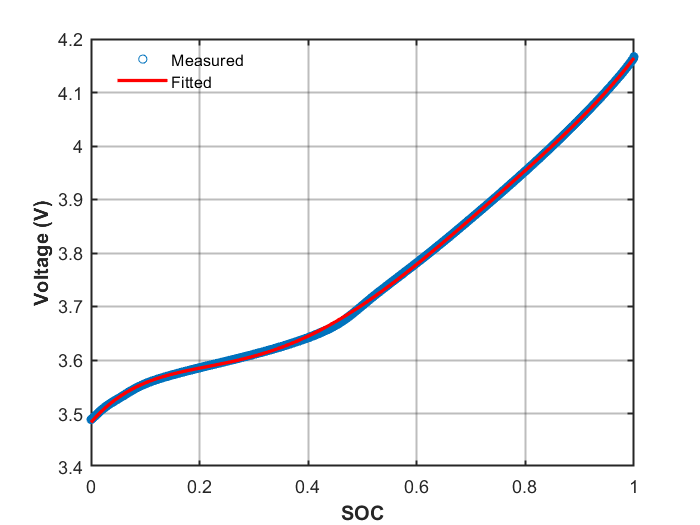
\includegraphics[width=0.4\textwidth]{figures/DST_.png}
% \caption{E-SOC curve}
% \label{fig:figure1}
% \end{figure}

Then, since the actual system control and parameter identification are performed in the discrete time domain,
the continuous-time state equations need to be converted into discrete form.
Let the sampling period be $\Delta t$, and based on the forward Euler and exponential discretization methods, the discrete state update equations for the second-order RC model are obtained:
\begin{equation}
\begin{cases}
U_1(k+1) = \exp\left(-\dfrac{\Delta t}{R_1 C_1}\right) U_1(k) + R_1\left[1 - \exp\left(-\dfrac{\Delta t}{R_1 C_1}\right)\right]i(k) \\[10pt]
U_2(k+1) = \exp\left(-\dfrac{\Delta t}{R_2 C_2}\right) U_2(k) + R_2\left[1 - \exp\left(-\dfrac{\Delta t}{R_2 C_2}\right)\right]i(k) \\[10pt]
SOC(k+1) = SOC(k) - \dfrac{\eta \cdot i(t) \cdot \Delta t}{Q_n}
\end{cases}
\label{eq:discrete}
\end{equation}

Finally, in order to avoid the reliance of traditional experimental methods on sophisticated equipment and large amounts of prior data,
this study employs the Genetic Algorithm (GA) to conduct global parameter identification for the second-order RC equivalent circuit model.
Define the parameter vector
   $\theta = \left[R0,R_1, R_2, C_1, C_2, SOC_0\right]^T$
where $SOC_0$ is the initial state of charge.
Based on the least squares principle, construct a loss function aimed at minimizing the terminal voltage error:
\begin{equation}
J\left( \theta \right) =\sqrt{\frac{1}{N}\sum_{k-1}^N{\left[ U_{meas}\left( k \right) -U\left( k \right) \right]}^2}
\end{equation}
where $U_{meas}(k)$ is the measured voltage data at time $k$. $U(k)$ is the simulated voltage under the current parameters, and $N$ is the length of the data sequence.
The iterative optimization process based on GA is shown in \autoref{fig:figure1}:
\begin{figure}[htbp]
  \centering
  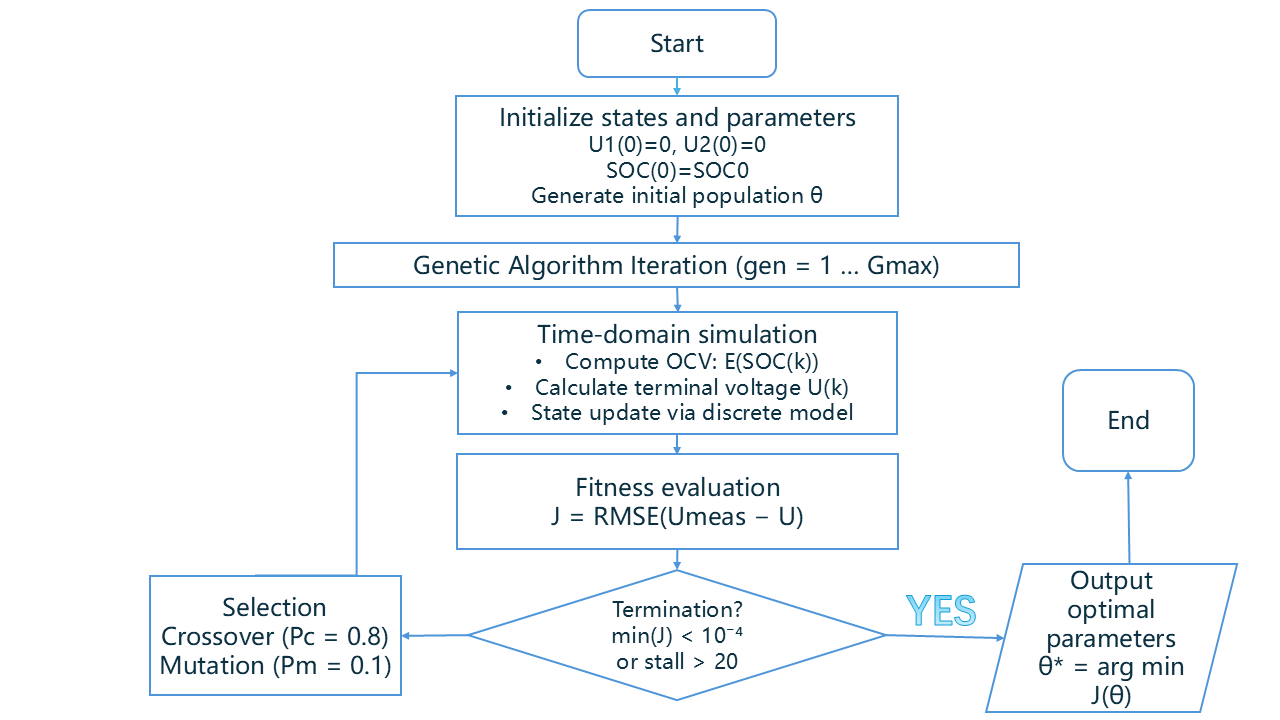
\includegraphics[width=0.7\textwidth]{figures/2.png}
  \caption{GA Parameter Identification Flowchart}
  \label{fig:figure1}
\end{figure}
\begin{itemize}
  \item Step 1: Initialize states, set initial conditions: $U_1(0)=0, U_2(0)=0$, initial state of charge $SOC(0)=SOC_0$.
   Generate the initial population according to the encoding scheme, each individual representing a candidate parameter set $\theta$.
  \item Step2: Time-domain simulation iteration. Based on the current $SOC(k)$, substitute into the fitted polynomial function to calculate the battery open-circuit voltage $E(SOC(k))$. Based on the current $E(SOC(k))$, substitute into the model to obtain the simulated battery voltage $U(k)$.
Then, state propagation, using the discrete state iteration equation \autoref{eq:discrete}, calculate the next moment $SOC\left(k+1\right)$, $U_1\left(k+1\right)$, $U_2\left(k+1\right)$ based on the current current and state variables.
  \item Step3: Genetic algorithm optimization,
Use the genetic algorithm to iteratively update the parameter vector. First, select excellent individuals based on the fitness function and perform crossover and mutation. Then repeat the previous steps until the error is less than the threshold or the maximum number of iterations is reached.
 \end{itemize}
% \begin{figure}[htbp]
% \centering
%     \centering
%     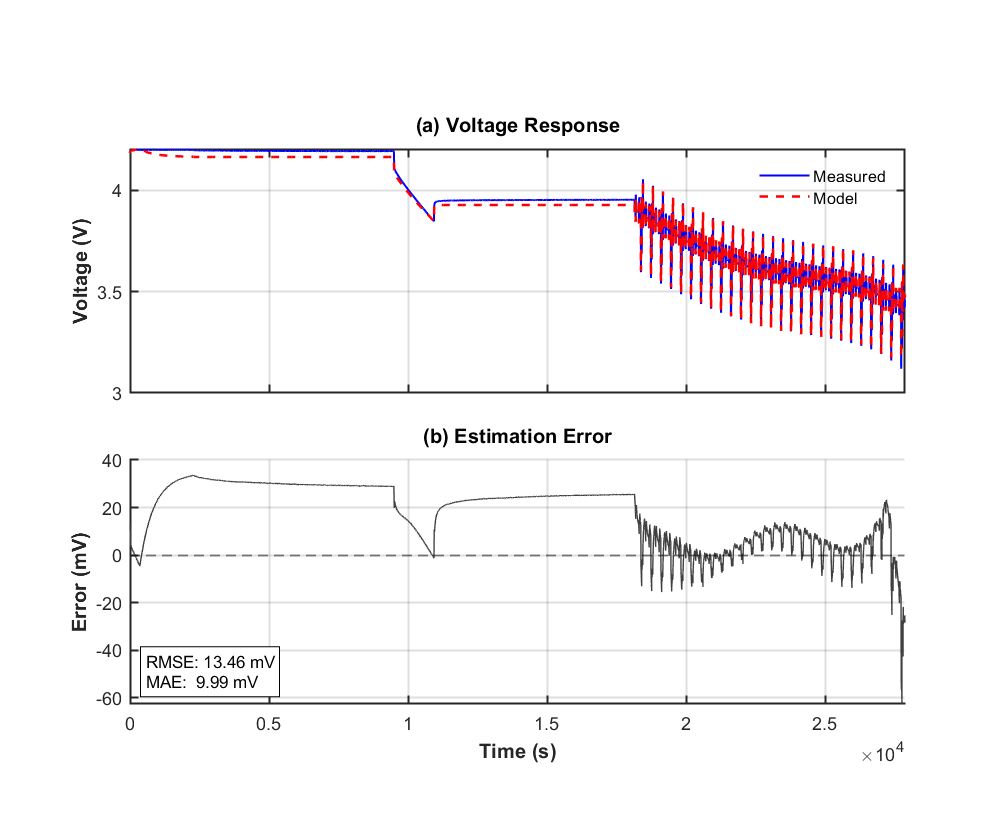
\includegraphics[width=0.5\textwidth]{figures/DST.png}
%     \caption{DST参数识别}
%     \label{fig:DST}
% \end{figure}
By using the publicly available DST dataset \cite{calce2024battery} for RC parameter identification, we ultimately obtained a set of optimal parameters as shown in \autoref{tab:parameter_identification}.
\begin{table}[htbp]
  \centering
  \caption{GA Parameter Identification Results Based on DST Conditions}
  \vspace{-0.4cm}
  \label{tab:parameter_identification}
  \begin{tabular}{cccccc}
    \toprule
    $R_0\ (\Omega)$ & $R_1\ (\Omega)$ & $C_1\ (\text{F})$ & $R_2\ (\Omega)$ & $C_2\ (\text{F})$ & $SOC_0\ (\%)$ \\
    \midrule
   0.05115&0.03658 &145.57 &0.01585 & 14017.48 & 95.65 \\
    \bottomrule
  \end{tabular}
  \\[6pt]  % 增加行间距
  \raggedright\footnotesize
  Note: Under these parameters, the identification error of the model: RMSE is $13.46 mV$, and MAE is $9.9 mV$.
\end{table}
\subsection{Model Validation}
To validate the accuracy of the established second-order $RC$ model,
we used a $100mA$ constant current discharge dataset \cite{android2024powervalues} for verification,
and the results are shown in \autoref{fig:DST_2}.
\begin{figure}[htbp]
    \centering
    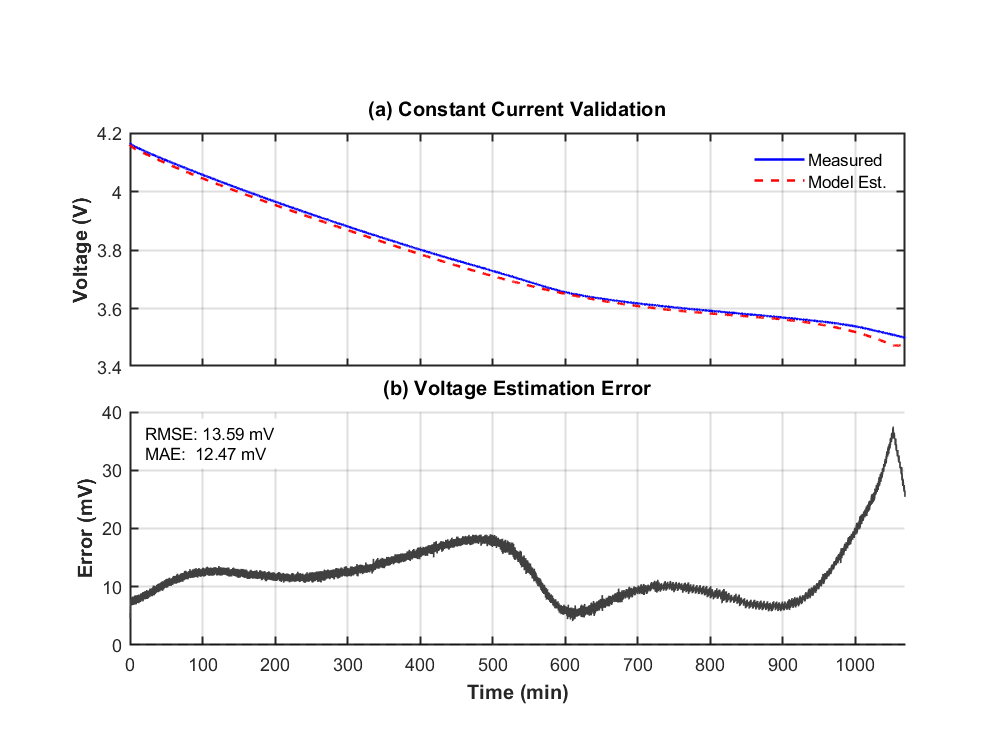
\includegraphics[width=0.6\textwidth]{figures/yanzheng.png}
    \caption{100mA Constant Current Discharge Test Validation}
    \label{fig:DST_2}
\end{figure}
\autoref{fig:DST_2}(a) shows the comparison between the measured voltage and the model estimated voltage,
\autoref{fig:DST_2}(b) presents the voltage estimation error throughout the discharge process.
The results indicate that the model estimates are highly consistent with the measured values during the entire discharge process,
the two curves almost completely overlap.
From the statistical characteristics of the error, except for the abnormal fluctuations at the end of the discharge, the error remains within $±15mV$ for most of the time,
with a root mean square error (RMSE) of $13.59mV$.

The above validation results indicate that the proposed equivalent circuit model combined with genetic algorithm parameter identification,
has sufficient accuracy for remaining time-to-empty prediction under real working conditions,
while also ensuring reliable SOC estimation across diverse usage scenarios.

\section{Time-to-Empty Prediction Model}
\subsection{Model Establishment}
Based on the comprehensive model established in the first question that couples multi-scenario application power and temperature effects, in order to achieve power prediction,
we use the Unscented Kalman Filter (UKF) algorithm for online estimation and prediction of battery SOC.
\subsubsection{State Space Model Construction}
To describe the dynamic characteristics of the battery, a state space model is constructed. The state vector is defined as $\mathbf{x}_k=[U_{1,k},U_{2,k},SOC_k]^T$, and the observed variable is the battery terminal voltage $y_k=U_k$.
\subsubsection*{UKF Prediction Algorithm Design}
The state estimation framework based on UKF (Unscented Kalman Filter) processes the strong nonlinear OCV-SOC relationship in the battery model through the \textbf{Unscented Transformation (UT)}. The core idea is to use a finite number of sigma points to accurately capture the mean and covariance of the state distribution, thereby achieving Bayesian recursive estimation. The specific implementation is divided into the following three stages:

\textbf{Stage 1: Sigma Point Generation and State Prediction}

First, based on the posterior estimate $\widehat{{x}}_{k-1}$ and its error covariance matrix $P_{k-1}$ at time $k-1$, $2L+1$ sigma points are deterministically sampled (with $L=3$ being the state dimension):
\begin{equation}
\begin{cases}
{X}_{0,k-1} = \widehat{{x}}_{k-1}, \\
{X}_{i,k-1} = \widehat{{x}}_{k-1} + \left(\sqrt{(L+\lambda)\mathbf{P}_{k-1}}\right)_i, & i = 1, \ldots, L, \\
{X}_{i,k-1} = \widehat{{x}}_{k-1} - \left(\sqrt{(L+\lambda)\mathbf{P}_{k-1}}\right)_{i-L}, & i = L+1, \ldots, 2L.
\end{cases}
\end{equation}
Here, $\lambda$ is the scaling parameter that controls the range of the sampling point distribution. These Sigma points are substituted into the discrete state equation for propagation, resulting in the prior state estimate $x_k^-$ and the prior covariance $P_k^-$:
\begin{equation}
  \begin{cases}
x_k^- = \sum_{i=0}^{2L} W_m^{(i)} X_{i,k|k-1}\\ P_k^- = \sum_{i=0}^{2L} W_c^{(i)} [X_{i,k|k-1} - \hat{x}_{k-1}][X_{i,k|k-1} - \hat{x}_{k-1}]^T + Q_k
  \end{cases}
\end{equation}
Here, $Q_k$ is the process noise covariance, representing model uncertainty.

\textbf{Stage 2: Measurement Prediction and Statistical Characteristic Extraction}

The predicted sigma points are mapped to the measurement space through the nonlinear observation equation $h(\cdot)$, calculating the predicted terminal voltage $h_{i,k}=E(X_{SOC})-I_kR_0-X_{U_1}-X_{U_2}$, thereby obtaining the predicted measurement mean $\hat{y}_k$.
\begin{equation}
{\hat{y}}_k=\sum_{i=0}^{2L}{W_m^{(i)}h_{i,k}} 
\end{equation}
To provide statistical basis for subsequent correction, the measurement innovation covariance $S_k$ and the state-measurement cross covariance $P_{xy,k}$ need to be calculated:
\begin{equation}
\begin{cases}
  S_k=\sum_{i=0}^{2L}{W_c^{(i)}[h_{i,k}-}{\hat{y}}_k][h_{i,k}-\hat{y}_k]^T+R_k,\\
  P_{xy,k}=\sum_{i=0}^{2L}{W_c^{(i)}[X_{i,k|k-1}-{\hat{x}}_k^-}][h_{i,k}-\hat{y}_k]^T.
\end{cases}
\end{equation}
Here, $R_k$ is the measurement noise covariance, reflecting the accuracy of the voltage sensor.

\textbf{Stage 3: Kalman Gain and State Correction}

Based on the minimum mean square error criterion, the optimal Kalman gain $K_k=P_{xy,k}S_k^{-1}$ is calculated. Using the residual between the actual measurement $U_{meas,k}$ and the predicted value $\hat{y}_k$, the prior estimate is corrected to obtain the posterior state $\hat{x}_k$ and the updated covariance $P_k$:
\begin{equation}
  \begin{cases}
    \hat{x}_k={\hat{x}}_k^-+K_k(U_{meas,k}-{\hat{y}}_k),\\
    P_k=P_k^--K_kS_kK_k^T.
  \end{cases}
\end{equation}
At this point, a complete filtering cycle has been completed. The third component in $\hat{x}_k$ represents the optimal SOC estimation after being corrected by the voltage feedback.
\subsubsection{Battery Life Model}
Unlike the short-term variations in internal resistance, battery life degradation is an irreversible cumulative process.
According to electrochemical kinetics principles, the rate of side reactions inside the battery also follows the Arrhenius equation.
Higher temperatures lead to larger reaction rate constants, causing the battery health state (SOH) to decline faster.
We establish a differential life model based on the Arrhenius equation.

First, the relationship between the battery aging rate and temperature is:
\begin{equation}
  k_{\text{aging}}(T) = k_{\text{ref,aging}} \cdot \exp\left[\frac{E_{a,\text{aging}}}{k}\left(\frac{1}{T_{\text{ref}}} - \frac{1}{T(t)}\right)\right]
\label{eq:aging}
\end{equation}
Here, $E_{a,aging}=52J/mol$\cite{Ecker2014CalendarCycleLife} is the activation energy for aging.

Next, considering the accelerating effect of current on side reactions, the differential equation for SOH is:
\begin{equation}
  \frac{dSOH}{dt}=-k_{aging}(T)\ast|i(t)|
\end{equation}

Finally, battery aging and its life degradation will in turn affect the battery's baseline internal resistance. Therefore, the internal resistance correction model after aging is considered as:
\begin{equation}
  R_{total}(t)=R(T)\ast(1+\alpha(1-SOH(t)))
\end{equation}
Here, $\alpha$ is the internal resistance growth coefficient, taken as 1.5 in this study.
Battery aging mainly manifests as the loss of active lithium ions and active materials. According to the definition of SOH, the maximum available chemical capacity after aging is also linearly related to SOH. The actual effective capacity of the battery at any time t and temperature T is:
\begin{equation}
  Q_n(t,T)=Q_{max}\cdot SOH(t)\cdot\eta_T(T)
\end{equation}
Therefore, the differential equation for the final battery state of charge under the influence of battery life also needs to introduce the correction of SOH. As SOH decreases, the denominator becomes smaller, and the same discharge current will cause SOC to decrease faster.
\begin{equation}
  \frac{d(SOC)}{dt}=-\frac{i(t)}{Q_{max}\cdot S O H(t)\cdot\eta}
\end{equation}

\subsection{Results Analysis}
\subsubsection*{Scenario Definition}
In order to study the power consumption and performance of the battery under different usage scenarios, we selected four typical usage scenarios ,the corresponding parameter configurations are shown in \autoref{tab:usage_scenarios_transposed}: 

\textbf{1. Low-power standby:} 
CPU utilization is the lowest, the screen is turned off, the GPS module is deactivated, only the basic network connection is maintained, and background tasks run intermittently to extend the system's standby life.

\vspace{-3pt}
\textbf{2. Video playback:} 
CPU load is moderate, screen brightness is increased to ensure the viewing experience, the network continues to work to ensure streaming media playback, and background tasks are still allowed to run.

\vspace{-3pt}
\textbf{3. Real-time navigation:} 
The device handles GPS positioning, map rendering, and network-assisted positioning simultaneously. The CPU load is high, the screen is fully lit, the data exchange volume is low, only the network signal connection is guaranteed, and power consumption significantly increases.

\vspace{-3pt}
\textbf{4. High-performance gaming:} 
CPU operates at full load, screen brightness is at its maximum, background tasks are blocked to ensure front-end performance, the network is stable and maintains moderate data synchronization, achieving a smooth interactive gaming experience.
\begin{table}[htbp]
\centering
\caption{Transposed layout of typical smartphone usage scenarios and key parameters}
\vspace{-0.4cm}
\label{tab:usage_scenarios_transposed}
\begin{tabularx}{\textwidth}{lXXXX}
\toprule
\textbf{Parameter} & \textbf{Standby} & \textbf{Video } & \textbf{Navigation} & \textbf{Gaming} \\
\midrule
 $u$ & 0.1 & 0.4 & 0.7 & 1.0 \\
$B$ & 0 & 0.6 & 1.0 & 1.0 \\
 GPS & Off & Off & On & Off \\
 $S_{signal}$ & 0.8 & 0.9 & 0.4 & 1.0 \\
 $D_{throughput}$ & 0.0 & 0.8 & 0.2 & 0.6 \\
Background Tasks & Intermittent pulses & Allowed & Allowed & Blocked \\
\bottomrule
\end{tabularx}

\end{table}




\subsubsection*{Prediction Results}
First, the short-term and long-term impacts of different usage scenarios on battery performance are evaluated. The SOC decline rates and long-term SOH degradation characteristics under the four typical scenarios are obtained, as shown in \autoref{fig:scenario_impact_comparison}.

\autoref{fig:fig_1_2} indicates that the SOC decline rates exhibit clear stratification and time-varying behavior across scenarios. In the Standby mode, the dissipation rate remains nearly constant at approximately 8\%/hour throughout the discharge process. In contrast, the three medium-to-high load scenarios (Video, Navigation, and Gaming) show progressively increasing dissipation rates over time.

Specifically, the Video scenario starts at about 40\%/hour and gradually increases to 46\%/hour after 100 minutes, corresponding to an increase of approximately 15\%. The Navigation and Gaming scenarios impose higher loads, where thermal accumulation becomes significant as usage time increases. The heat generated by the phone system raises the battery temperature, accelerates discharge, and leads to a more pronounced depletion trend. The dissipation rate in Navigation increases from 57\%/hour to 67\%/hour, while Gaming rises sharply from 68\%/hour to nearly 78\%/hour, with a slope markedly steeper than that of Video.

\begin{figure}[htbp]
\centering
\begin{subfigure}{0.48\textwidth}
\centering
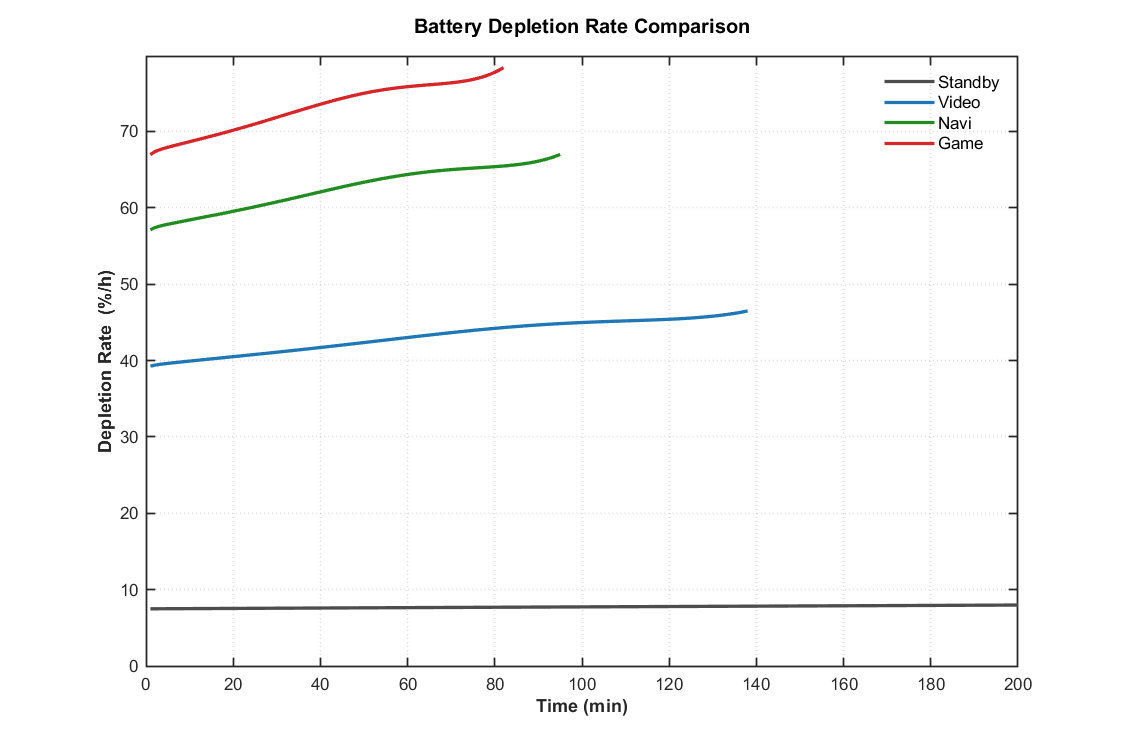
\includegraphics[width=\linewidth]{figures/p2_6.png}
\caption{Comparison of SOC decline rates under different usage scenarios (single discharge)}
\label{fig:fig_1_2}
\end{subfigure}
\hfill
\begin{subfigure}{0.48\textwidth}
\centering
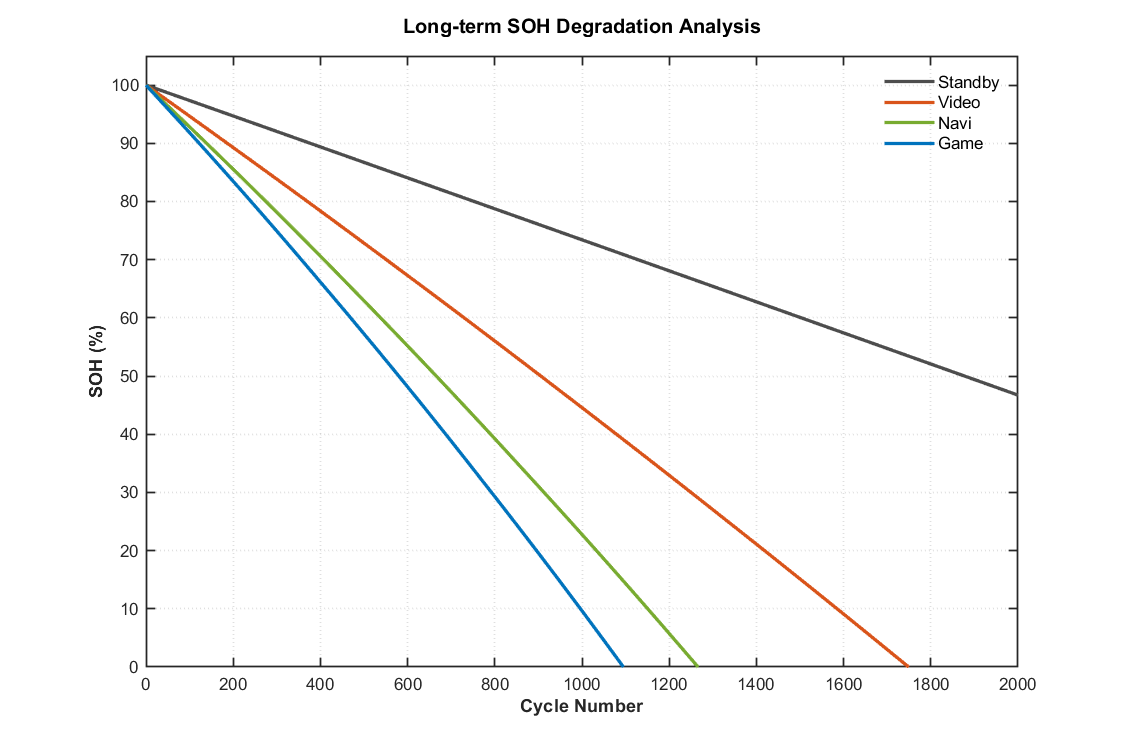
\includegraphics[width=\linewidth]{figures/p2_8.png}
\caption{Comparison of SOH degradation under different usage scenarios (cycle aging)}
\label{fig:fig_6}
\end{subfigure}
\caption{Short-term and long-term impacts of usage scenarios on battery performance}
\label{fig:scenario_impact_comparison}
\end{figure}

As shown in \autoref{fig:fig_6}, the SOH degradation in all four scenarios follows a layered, 
approximately linear declining trend, with substantially different slopes. 
The Gaming scenario exhibits the fastest degradation, reaching the end-of-life threshold (SOH $\approx 0\%$) after approximately 1100 cycles.
This behavior is attributed to sustained high-current discharge and elevated battery temperature caused by intensive CPU operation. 
According to \autoref{eq:aging}, high temperature significantly accelerates side reaction rates, thereby exacerbating battery aging.

The Navigation scenario shows slightly lower heat accumulation than Gaming but remains much higher than light usage due to continuous GPS RF power consumption and screen illumination,
 resulting in capacity depletion after approximately 1250 cycles.
 In the Video scenario, both current amplitude and operating temperature are lower than those in Gaming and Navigation, 
 leading to a gentler aging slope and a lifespan of approximately 1750 cycles,
  although still about 2.15 times faster than Standby. In contrast, 
  the Standby scenario operates under low current and near-room-temperature conditions,
   yielding an extremely small aging rate constant with nearly negligible side reactions. 
   Even after 2000 cycles, the SOH remains at approximately 47\%, 
   representing the upper limit of battery life under ideal storage conditions.
Then, this paper predicts the battery SOC for the above four typical usage scenarios (Standby, Video, Navi, Game)
and four initial SOC states (100\%, 80\%, 50\%, 20\%), a total of 16 combinations,
as shown in \autoref{fig:model_prediction}, with specific values and prediction results shown in \autoref{tab:prediction_results}.

\begin{figure}[htbp]
  \centering
  \begin{subfigure}[b]{0.45\textwidth}
    \centering
    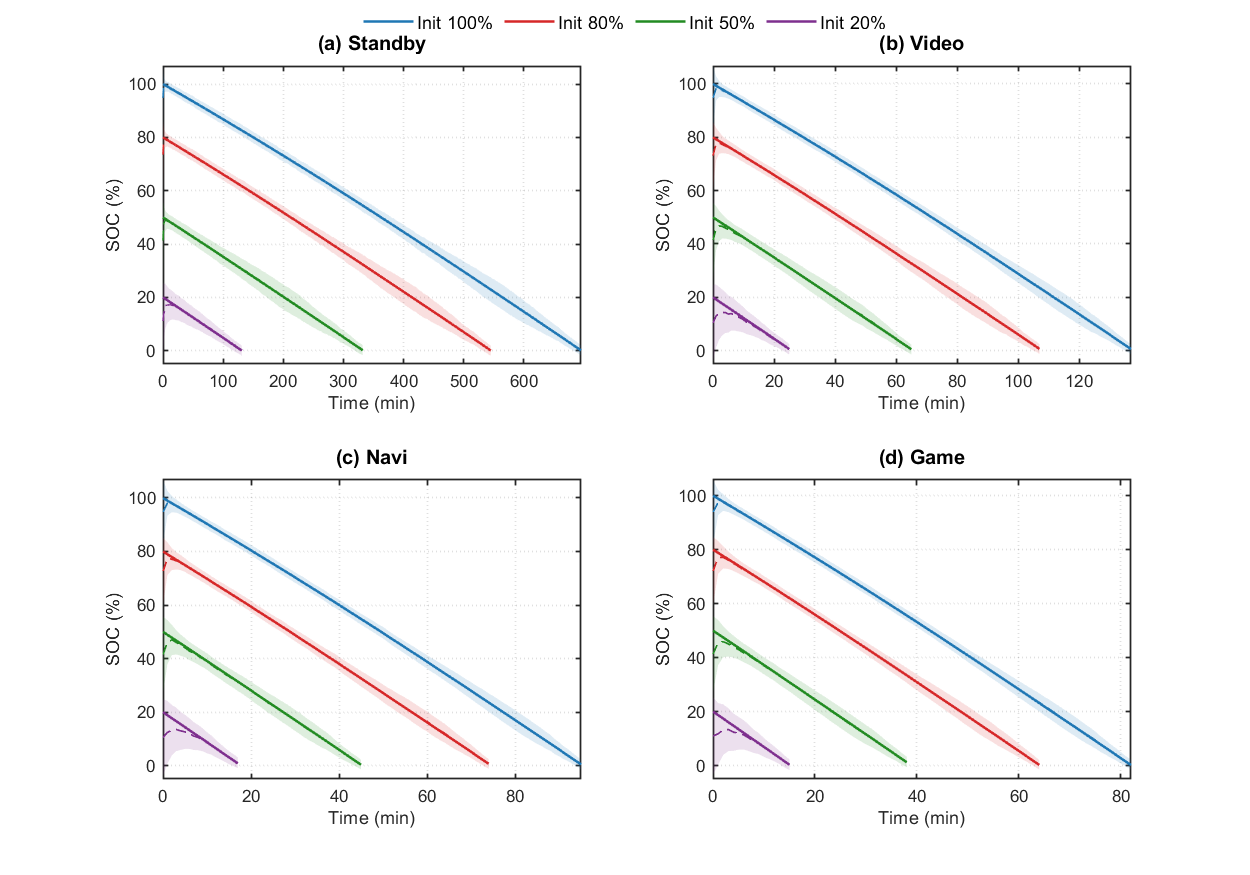
\includegraphics[width=\textwidth]{figures/n3.png}
    \caption{SOC prediction curves in different scenarios}
    \label{fig:soc_prediction}
  \end{subfigure}
  \hfill  
  \begin{subfigure}[b]{0.45\textwidth}
    \centering
    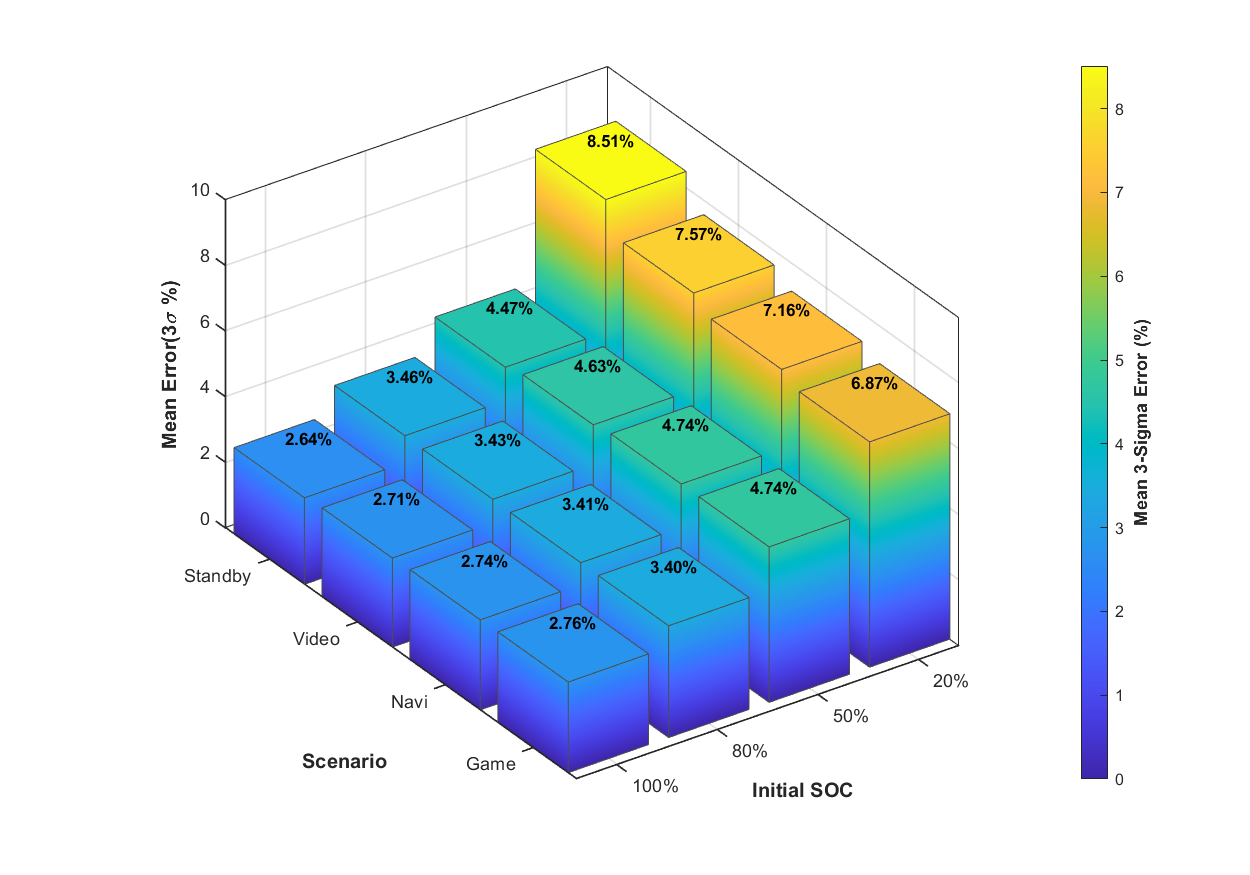
\includegraphics[width=\textwidth]{figures/n4.png}
    \caption{Average $3\sigma$ prediction error distribution}
    \label{fig:prediction_error}
  \end{subfigure}
  \caption{Model prediction performance analysis under different scenarios and initial SOCs}
  \label{fig:model_prediction}
\end{figure}

\begin{table}[htbp]
\centering
\caption{Discharge time  and the average $3\sigma$ prediction error}
\vspace{-0.4cm}
\label{tab:prediction_results}
\resizebox{\textwidth}{!}{%
\begin{tabular}{c|cc|cc|cc|cc}
\hline
\multirow{2}{*}{\textbf{Initial SOC}} & \multicolumn{2}{c|}{\textbf{Standby}} & \multicolumn{2}{c|}{\textbf{Video}} & \multicolumn{2}{c|}{\textbf{Navi}} & \multicolumn{2}{c}{\textbf{Game}} \\ \cline{2-9}
                                   & Time (min) & Error (\%) & Time (min) & Error (\%) & Time (min) & Error (\%) & Time (min) & Error (\%) \\ \hline
100\%                              & 700       & 2.66     & 130       & 2.72     & 90        & 2.76     & 81        & 2.77     \\
80\%                               & 550       & 3.46     & 107       & 3.43     & 72        & 3.41     & 63        & 3.40     \\
50\%                               & 330       & 4.51     & 65        & 4.68     & 43        & 4.74     & 39        & 4.74     \\
20\%                               & 120       & 8.50     & 25        & 7.39     & 18        & 7.20     & 15        & 6.96     \\ \hline
\end{tabular}%
}
\end{table}
From the SOC prediction curves, the model successfully captures battery discharge characteristics under different scenarios. Under the same initial SOC, battery endurance decreases with increasing load power; under the same load, endurance shortens with decreasing initial SOC. The shaded areas represent the $3\sigma$ confidence intervals, where $\sigma$ is the SOC prediction standard deviation, and the width intuitively reflects prediction accuracy.

Model performance is further quantified via the three-dimensional bar chart of average $3\sigma$ prediction error. The color gradient from blue to yellow reflects increasing error. Results show that initial SOC is the dominant factor: prediction error rises significantly from 100\% to 20\% initial SOC due to the flat OCV-SOC curve in the low SOC region, where reduced voltage sensitivity amplifies SOC deviations from voltage noise, increasing $\sigma$ and the $3\sigma$ interval.

Considering usage scenarios, at 20\% initial SOC, Standby has the largest error (8.50\%) and Game the smallest (6.96\%), reflecting the amount of observation information: Game features significant voltage changes for better prediction correction, while Standby’s slow changes limit measurement updates. At high SOC (100\% and 80\%), errors are small and similar (2.6\%-3.4\%), indicating higher voltage sensitivity improves accuracy and reduces scenario dependence. Overall, across 16 operating conditions, the average $3\sigma$ prediction error ranges from 2.66\% to 8.50\%, demonstrating the model reliably predicts SOC under complex loads and environments.

Next, we conducted a study on Time-to-Empty Prediction starting from different initial SOCs in dynamic usage scenarios, and systematically evaluated the prediction capability of the constructed model as well as the error convergence characteristics of the Unscented Kalman Filter (UKF) algorithm. The results are shown in \autoref{fig:fig_322}.
\begin{figure}[htbp]
  \centering
  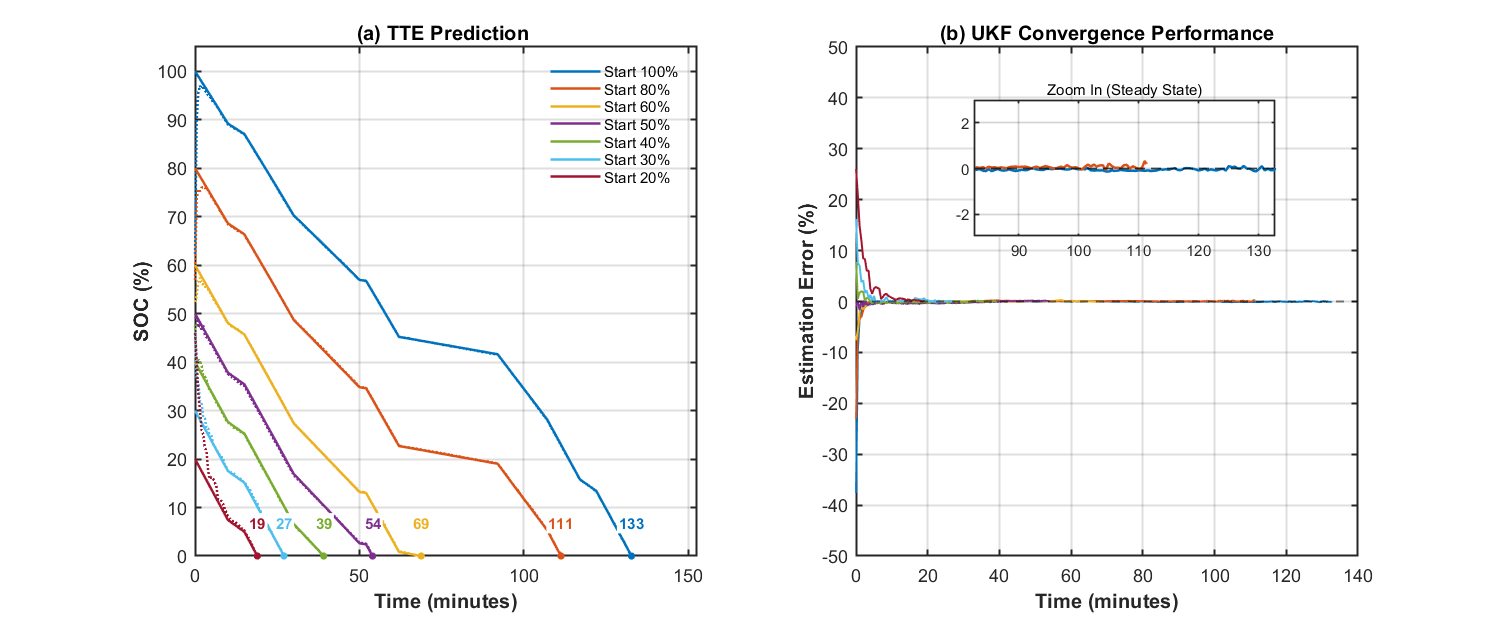
\includegraphics[width=0.8\textwidth]{figures/n2.png}
  \caption{Evaluation results of Time-to-Empty Prediction in dynamic scenarios}
  \label{fig:fig_322}
\end{figure}
The left figure shows the Time-to-Empty Prediction starting from different initial SOCs in dynamic scenarios,
while the right figure illustrates the error convergence process of the UKF algorithm with the initial estimate fixed at 50\%.
These two subplots validate the model's predictive capability and the algorithm's adaptive performance from different perspectives.

We summarize the Time-to-Empty prediction results under different initial SOC conditions, considering dynamic thermal effects and network connectivity, in \autoref{tab:tte_prediction}.
It can be seen that as the initial SOC decreases, the average discharge rate shows a gradually increasing trend,
indicating that the energy consumption of the battery in the low SOC range is significantly accelerated.
The physical origin of this phenomenon lies in the superposition of multiple factors. First, the internal resistance of the battery increases as SOC decreases, resulting in more energy being lost in the form of heat.
Second, when the SOC is low, the battery terminal voltage decreases, and to maintain constant power output, the current must increase, further exacerbating energy consumption.
\vspace{-0.3cm}
\begin{table}[htbp]  
\centering
  \caption{Prediction results of Time-to-Empty under different SOC levels}
  \label{tab:tte_prediction}
  \vspace{-0.4cm}
  \begin{tabular}{@{}ccc@{}}
    \toprule
    Initial SOC (\%) & Time-to-Empty (min) & Avg. Discharge Rate (\%/min) \\
    \midrule
    100 & 133 & 0.75 \\
    80  & 111 & 0.72 \\
    60  & 69  & 0.87 \\
    50  & 54  & 0.93 \\
    40  & 39  & 1.03 \\
    30  & 27  & 1.11 \\
    20  & 19  & 1.05 \\
    \bottomrule
  \end{tabular}
\end{table}

The right figure illustrates the error convergence process of the UKF algorithm under significant initial state estimation deviations,
used to evaluate the robustness of the state estimation algorithm.
In the experimental design, all tests fixed the initial SOC estimate at 50\%,
with initial estimation error ranging from +50\% to -30\%.
From the overall characteristics of the error curves, the UKF algorithm demonstrates good convergence performance under all test conditions.
Under different initial error scenarios, the estimation error can rapidly converge to within ±2\% in about 5-10 minutes,
and further stabilize within ±1\%. This indicates uniform estimation accuracy across all SOC ranges,
validating the robustness and adaptability of the UKF algorithm.

Finally, we conducted a study on the established capacity degradation model,
and obtained the relationship between battery capacity and cycle count through MATLAB simulation.
The results are shown in \autoref {fig:fig_3}.
\begin{figure}[htbp]
  \centering
  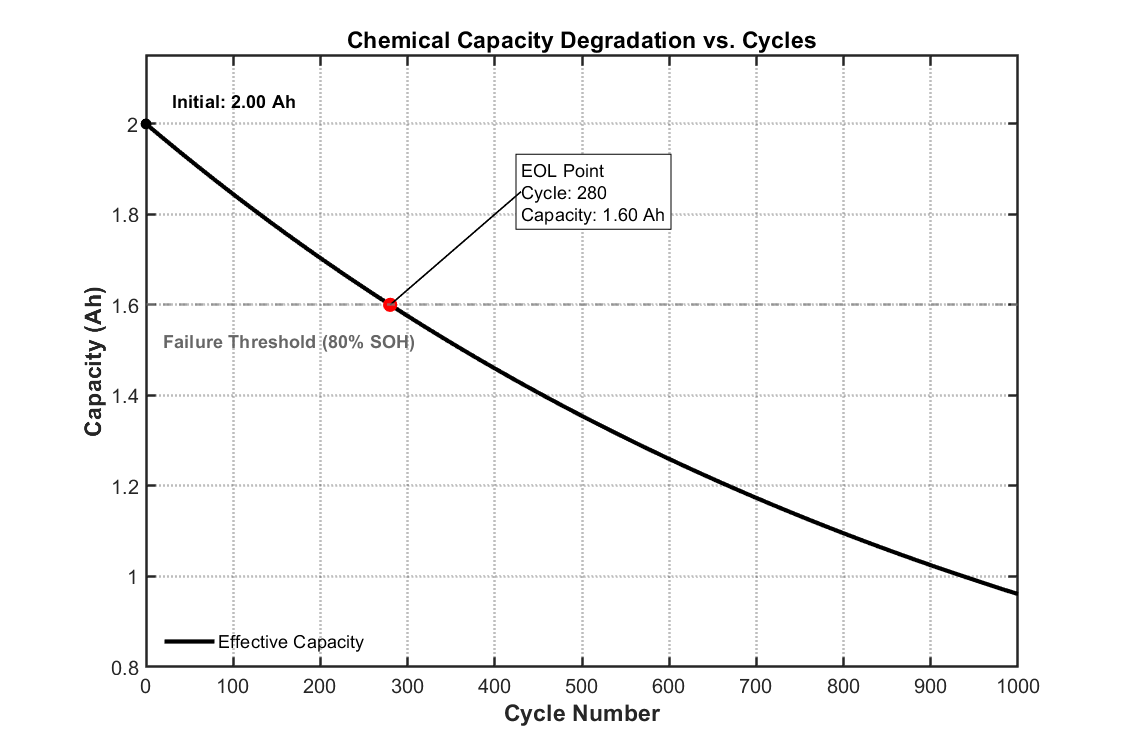
\includegraphics[width=0.5\textwidth]{figures/p2_9.png}
  \caption{Capacity vs. Cycle Count Curve}
  \label{fig:fig_3}
\end{figure}

The results show that the effective capacity of the battery starts at an initial value of $2.00 Ah$ and exhibits an approximately linear decline with increasing cycle count.
The battery loses about $1.04 Ah$ of capacity over 1000 cycles, with an average degradation of 0.052\% of the initial capacity per cycle.
According to the industry standard 80\% EOL definition,
the model predicts that the battery reaches its end-of-life point (capacity 1.60 Ah, marked by the red dot in the figure) at about 280 cycles,
providing a quantitative basis for battery replacement strategies and warranty period design for smartphone manufacturers.
\section{Sensitivity Analysis}
\subsection{The impact of different environmental temperatures on the battery life}
To evaluate the impact of environmental temperature on battery performance, we selected three typical environmental temperature conditions: 0°C, 20°C, and 35°C, and conducted SOC decay tests under four usage scenarios.
The results are shown in \autoref {fig:fig_temp}.
\begin{figure}[htbp]
  \centering
  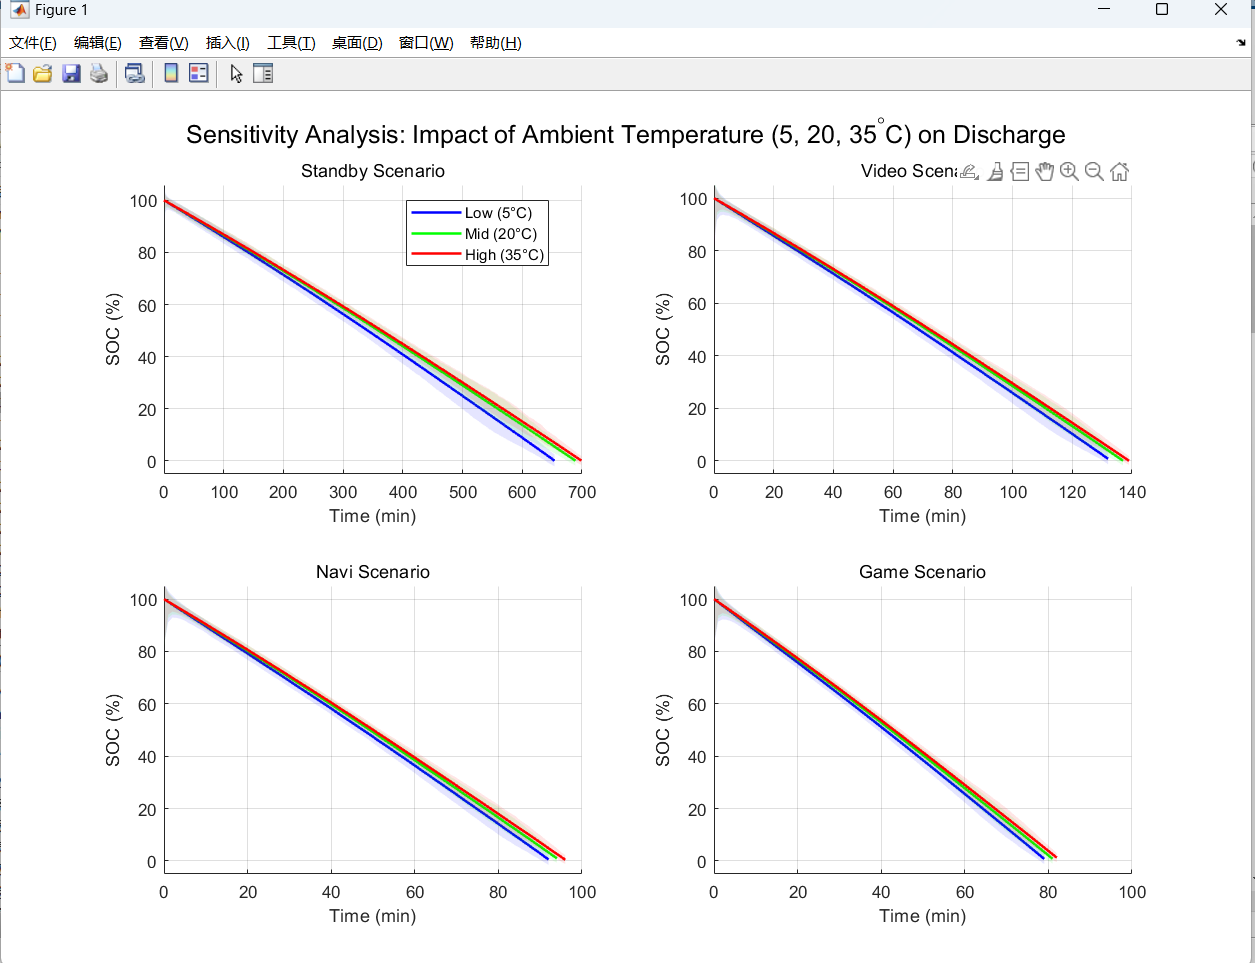
\includegraphics[width=0.8\textwidth]{figures/image_p3_1.png}
  \caption{SOC Decay Curves at Different Temperatures}
  \label{fig:fig_temp}
  \end{figure}

The results show that in any scenario, the lower the temperature, the faster the discharge speed.
For example, in the low-load standby scenario,
discharging at 5°C is the fastest, with the shortest battery life of approximately 650 minutes, while discharging at 20°C or 35°C is slower, with a battery life of approximately 700 minutes), with a variation of 7%.
However, this temperature sensitivity sharply decreases as the load increases. In high-load scenarios such as video (Video), navigation (Navi), and gaming (Game),
the curves representing the three temperatures almost completely overlap.
The physical root cause lies in the dominant effect of Joule heating. The internal heat generated by the large current discharge
causes the battery temperature to rapidly rise to a stable working temperature far above the ambient level. At this point, regardless of whether the initial ambient temperature is 5°C or 35°C,
the internal temperature trajectory of the battery during actual operation tends to be consistent, resulting in the rapid elimination of the temperature-dependent internal resistance
and the difference in effective capacity.
Therefore, the decisive role of user behavior on battery life far exceeds the influence of environmental temperature fluctuations.
\subsection{The impact of model coefficient $\beta_2$ on the model}
To quantitatively assess the sensitivity of the nonlinear coefficient $\beta_2$ in the CPU power consumption model and verify its validity under extreme operating conditions, boundary condition tests are conducted to determine a reasonable range of $\beta_2$.
The revised CPU power model is given by
\begin{equation}
P_{CPU}(t) = 0.1 + 2.28 \cdot u(t) + \beta_2 \cdot [u(t)]^2 .
\end{equation}

Under the maximum load condition ($u=1$), the predicted power is
\begin{equation}
P = 0.1 + 2.28 + \beta_2 .
\end{equation}
When $\beta_2 = 0.5$, the model yields $P_{CPU}=2.88$ W, which exactly matches the measured maximum power, validating the model accuracy at high load.

Under the minimum load condition ($u=0.1$), the predicted power is $P_{CPU}=0.333$ W, which is close to the measured value of 0.36 W, with an absolute error of 0.027 W, satisfying the requirements of sensitivity analysis.
These boundary condition results indicate that $\beta_2 = 0.5$ provides good fitting accuracy across the full load range.
To further assess the impact of $\beta_2$ on the overall battery performance prediction,
this paper selected two parameter settings: $\beta_2 = 0.2$ and $\beta_2 = 0.5$,
and conducted a comparative experiment on the complete discharge cycle under dynamic load.
The results are shown in  \autoref{fig:p3_4}.
\begin{figure}[htbp]
  \centering
  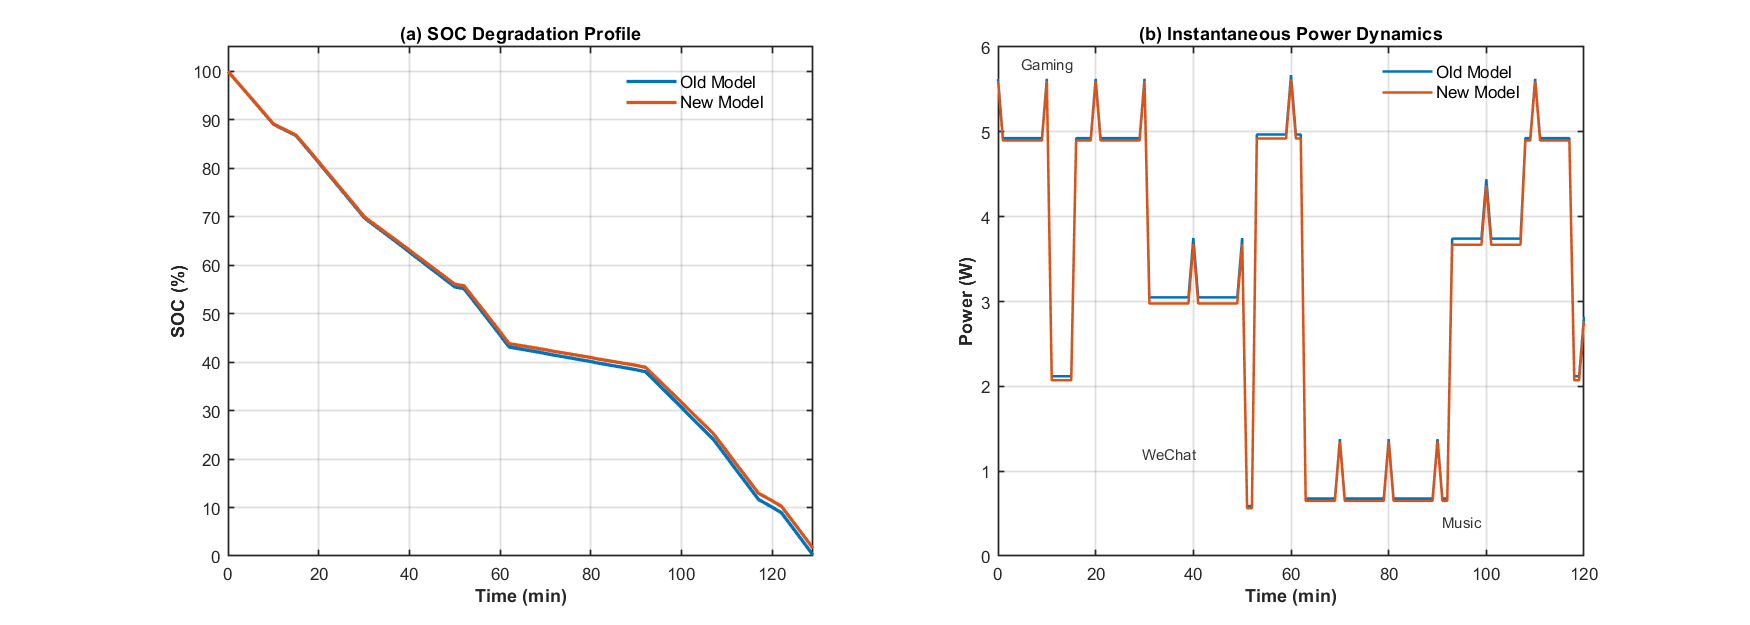
\includegraphics[width=1\textwidth]{figures/image_p3_4.png}
  \caption{SOC Decay Curves and Power Variation under Different $\beta_2$}
  \label{fig:p3_4}
\end{figure}

From the figure, it can be seen that during the complete SOC discharge cycle (about 120 minutes),
the SOC decay curves and power variation curves of the model under two different $\beta_2$ parameters are highly overlapping.
Although $\beta_2$ increases from 0.2 to 0.5, i.e., the nonlinear term is enhanced by 150\%,
the impact on total power consumption and endurance time is minimal,
mainly because in practical usage scenarios, the contribution of the quadratic term $\beta_2[u(t)]^2$ under different CPU utilization conditions is relatively small compared to the linear term $2.28u(t)$.
This result indicates that although $\beta_2$ is crucial for power prediction accuracy under boundary conditions,
the model exhibits a certain degree of robustness to this parameter in dynamic mixed load scenarios,
which facilitates the model's transferability across different devices and application scenarios.
\subsection{The impact of screen brightness on battery performance}
To evaluate the impact of screen brightness on battery performance,
this paper conducted comparative experiments under game mode and standby mode,
setting three brightness levels: 50\%, 75\%, and 100\%.
Figure \ref{fig:fig_brightness_comparison} shows the experimental results in both scenarios.
\begin{figure}[htbp]
\centering
\begin{subfigure}{0.45\textwidth}
    \centering
    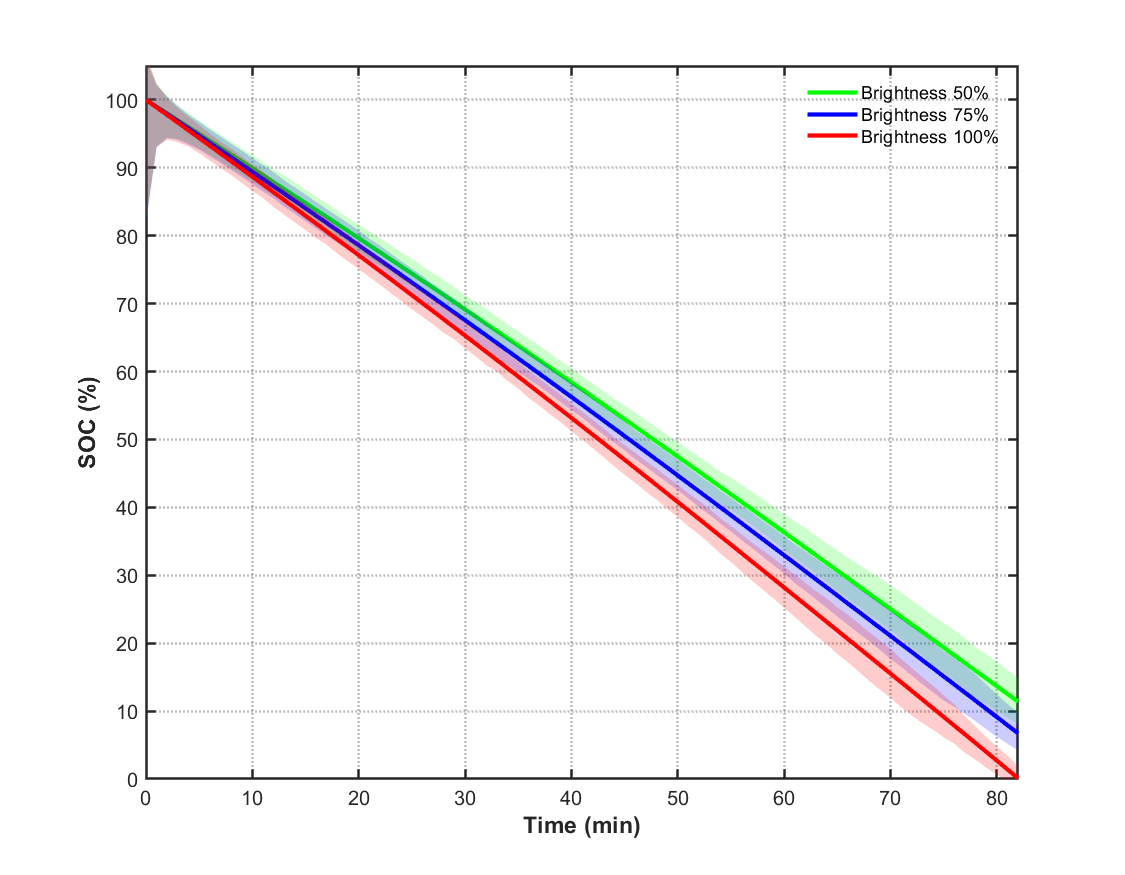
\includegraphics[width=\linewidth]{figures/image_p3_2.png}
    \caption{SOC Decay Curves under Different Brightness Levels (Game Scenario)}
    \label{fig:fig_brightness_soc}
\end{subfigure}
\hfill
\begin{subfigure}{0.45\textwidth}
    \centering
    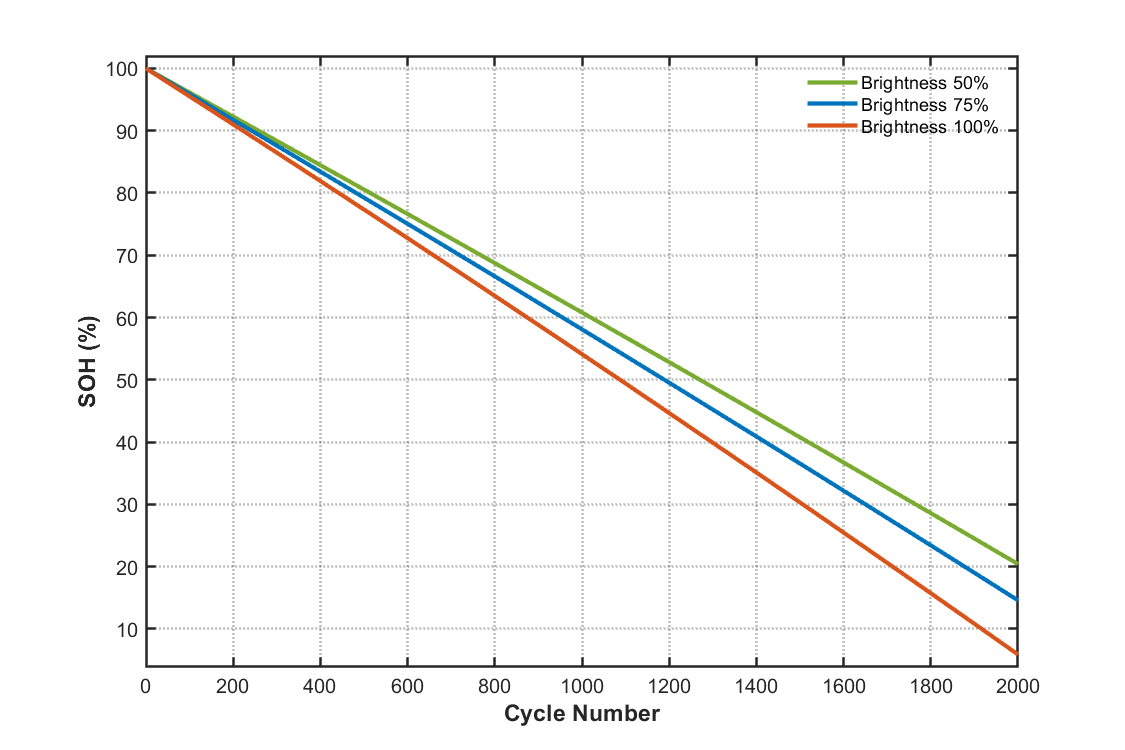
\includegraphics[width=\linewidth]{figures/image_p3_22.png}
    \caption{SOH Decay Curves under Different Brightness Levels (Standby Scenario)}
    \label{fig:fig_brightness_soh}
\end{subfigure}
\caption{Comparative Analysis of the Impact of Screen Brightness on Battery Performance}
\label{fig:fig_brightness_comparison}
\end{figure}

In the game scenario, since the CPU load dominates,
the impact of screen brightness on endurance time is relatively limited, showing diminishing marginal returns.
As shown in Figure \ref{fig:fig_brightness_soc},
when the screen brightness is reduced from 100\% to 50\%, the game endurance time only increases by about 10 minutes,
because the high computational intensity of the game scenario makes the CPU power consumption account for a larger proportion of the total power consumption,
and the reduction in screen power consumption partially offsets the improvement in overall endurance.
In contrast, the impact of screen brightness on the long-term health state of the battery is more significant in standby mode.
As shown in Figure \ref{fig:fig_brightness_soh},
the battery aging is most aggressive at 100\% brightness,
while it is slowest at 50\% brightness, with SOH remaining above 20\% after 2000 cycles.
In standby mode, the screen becomes the dominant load,
and since brightness is proportional to the square of the current,
high brightness settings directly accelerate the side reaction process based on the Arrhenius equation,
leading to increased accumulation of irreversible damage per cycle,
thereby having a profound impact on battery life.
\subsection{The impact of network throughput on battery performance}
To evaluate the impact of network data transmission intensity on battery performance,
this paper conducted sensitivity analysis under game mode and standby mode.
Figure \ref{fig:network_game} shows the short-term impact of different network throughput on SOC decay during game operation,
and Figure \ref{fig:network_standby} analyzes the long-term impact of network throughput on battery life in standby mode.
Three levels of network data transmission were set in both scenarios:
low data volume (D=0.1), medium data volume (D=0.5), and high data volume (D=1.0).
\begin{figure}[htbp]
    \centering
    \begin{subfigure}[b]{0.45\textwidth}
        \centering
        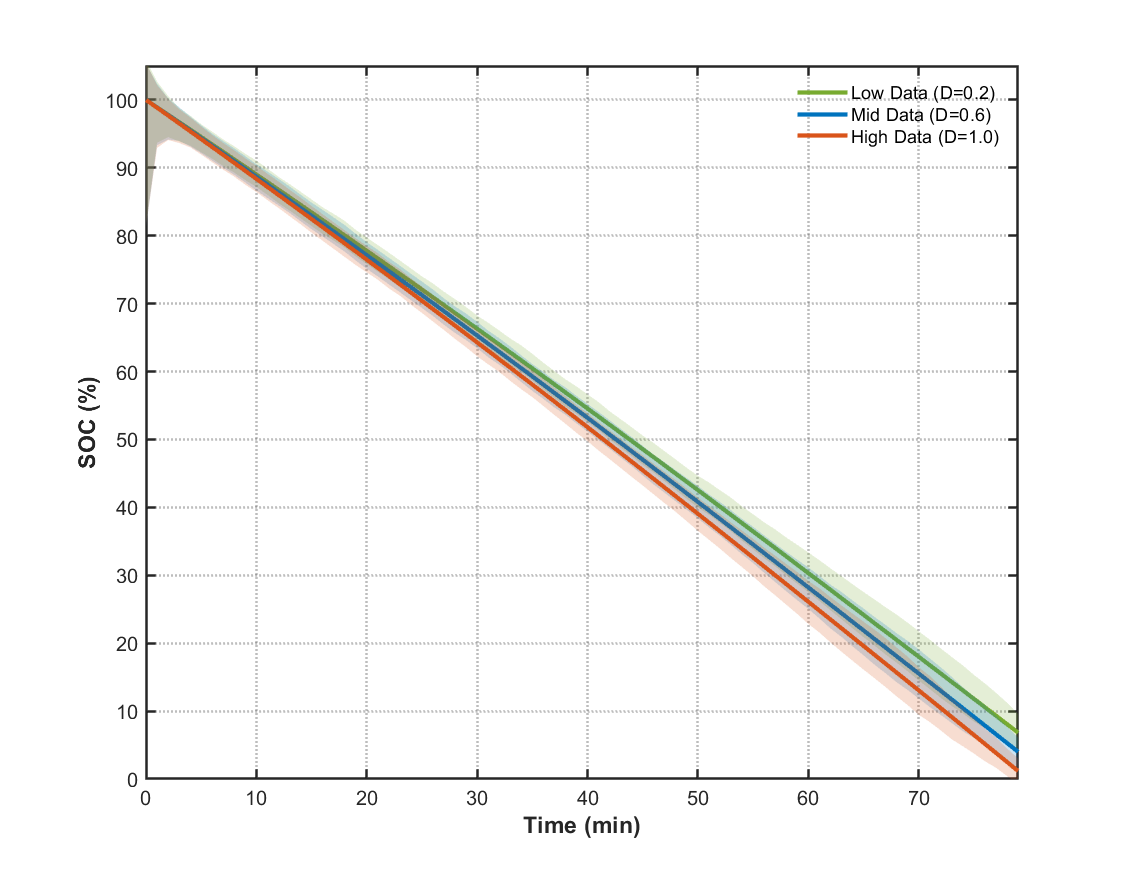
\includegraphics[width=\textwidth]{figures/sen1.png}
        \caption{Impact of Network Throughput on SOC in Game Mode}
        \label{fig:network_game}
    \end{subfigure}
    \hfill
    \begin{subfigure}[b]{0.45\textwidth}
        \centering
        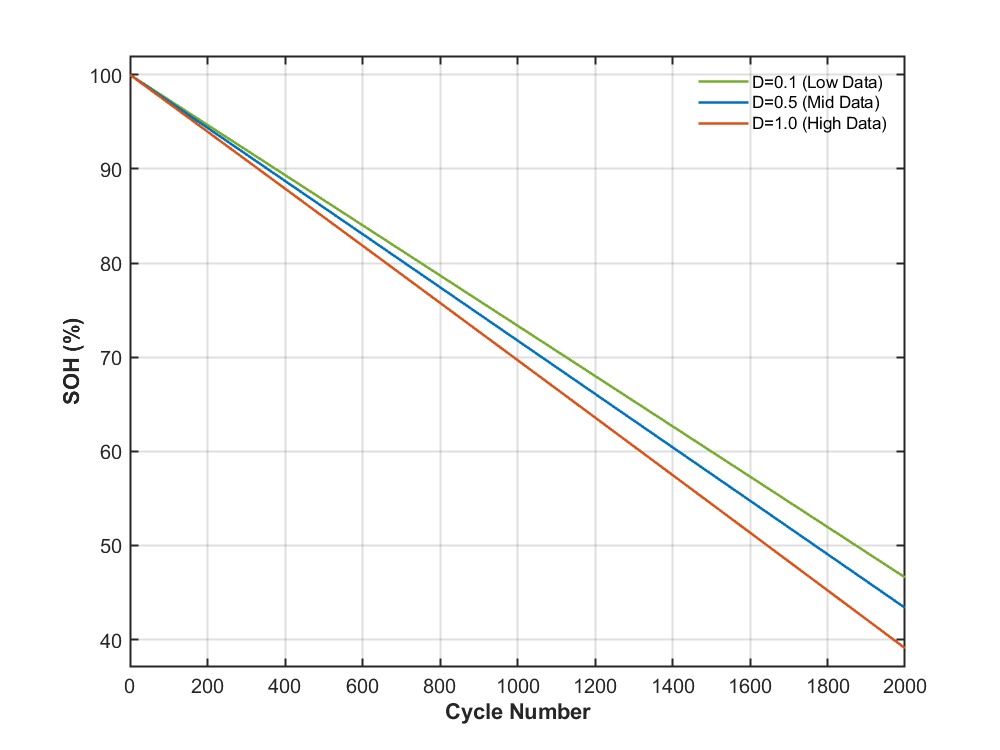
\includegraphics[width=\textwidth]{figures/sen2.png}
        \caption{Impact of Network Throughput on SOH in Standby Mode}
        \label{fig:network_standby}
    \end{subfigure}
    \caption{Comparative Analysis of the Impact of Network Throughput on Battery Performance}
    \label{fig:network_impact_comparison}
\end{figure}
During the initial discharge period (0-20 minutes), the three curves were almost completely overlapping.
However, as the discharge progressed to the later stage, the impact of network data volume on SOC gradually became apparent.
High data volume transmission (D=1.0) led to the fastest decline in SOC,
while low data volume transmission (D=0.1) showed the slowest decline in SOC.
This difference stems from the fact that the network transmission power consumption accounts for a relatively small proportion of the overall power consumption, and its cumulative effect becomes more pronounced over time.
In contrast, the long-term impact of network throughput in the standby mode on battery life is more persistent.
By 2000 cycles, it dropped to 39\%, 44\%, and 46\% respectively, with a battery life difference of approximately 6-7%.
The results indicate that in high-load scenarios, CPU and screen power consumption should be prioritized for optimization,
while in daily standby scenarios, attention should be focused on controlling network activities and background tasks. 
\subsection{Impact of Task Fluctuations on the Model}
To assess the impact of task fluctuations on the time prediction model, this paper designed a mixed usage scenario that included various task switches to simulate the behavior patterns of users in actual use.
The results are shown in \autoref{fig:dynamic_load_validation}.

From \autoref{fig:dynamic_power} real-time power consumption breakdown chart, it can be seen that the test process covered a high load stage with a total power of about 4.5-5.5W,
a medium load stage with a total power of about 3W,
a standby low power stage with a total power of less than 0.5W,
and moments of sudden power switching, forming a complex dynamic usage scenario.
Under such drastic power fluctuations,
the UKF estimated SOC curve in \autoref{fig:dynamic_soc} remains highly consistent with the true SOC curve,
with an average $3\sigma$ error of only 2.35\%,
indicating that the SOC estimation error is controlled within ±2.35\% at a 99.7\% confidence level,
demonstrating extremely high estimation accuracy.
At multiple load switching moments (such as 10, 15, 50, and 6 minutes),
the UKF estimation did not show significant deviation,
which can be attributed to its nonlinear filtering characteristics and real-time measurement update mechanism.
This dynamic load test fully validates the robustness of our UKF-based model in real complex usage scenarios,
maintaining high-precision estimation even in the face of frequent task switching and drastic power fluctuations.
\begin{figure}[htbp]
  \centering
  \begin{subfigure}[b]{0.43\textwidth}
    \centering
    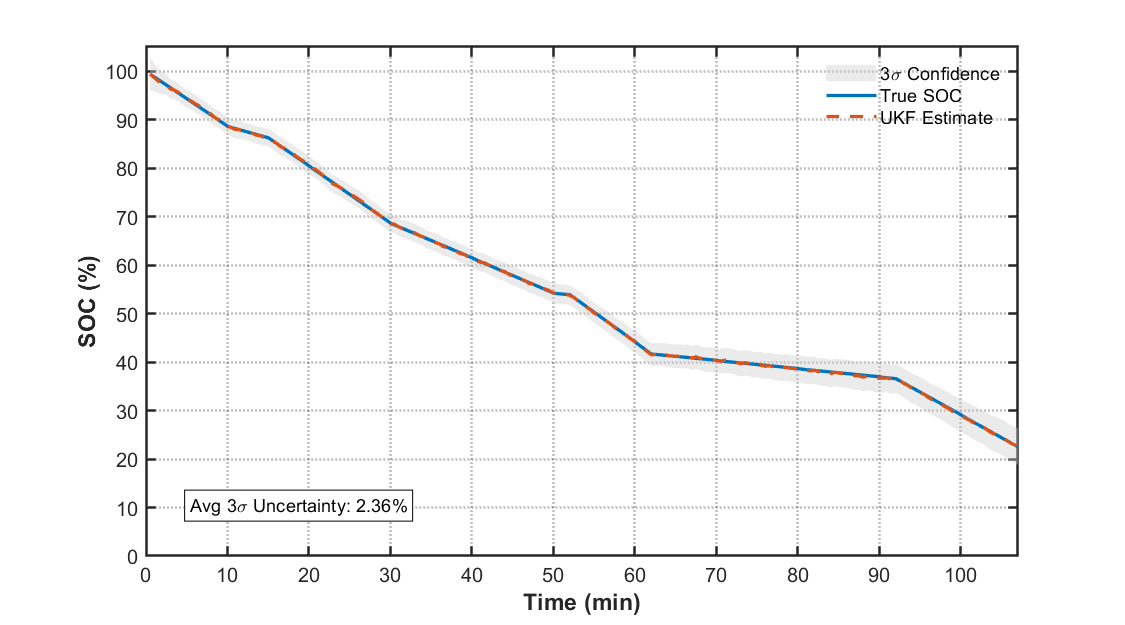
\includegraphics[width=\textwidth]{figures/image_p2_21.png}
    \caption{SOC Estimation  under Dynamic Load}
    \label{fig:dynamic_soc}
  \end{subfigure}
  \hfill
  \begin{subfigure}[b]{0.54\textwidth}
    \centering
    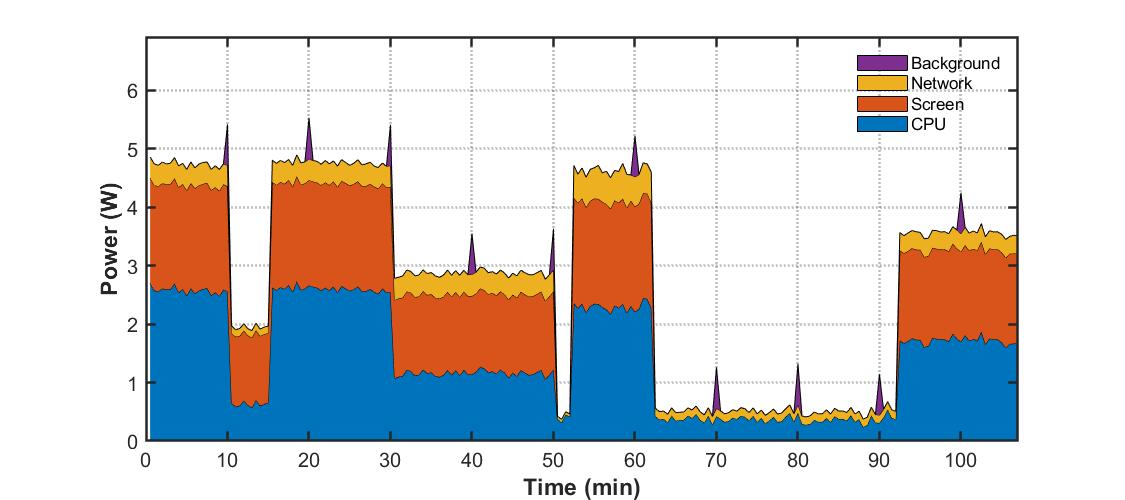
\includegraphics[width=\textwidth]{figures/image_p2_22.jpeg}
    \caption{Real-time Power Consumption Breakdown}
    \label{fig:dynamic_power}
  \end{subfigure}
  \caption{Impact of Task Fluctuations on the Model}
  \label{fig:dynamic_load_validation}
\end{figure}

\subsection{Impact of Internal Resistance Model on SOH Degradation Prediction}
To assess the impact of internal resistance model accuracy on battery health state (SOH) prediction,
this paper compared two different internal resistance modeling methods: a hybrid model considering aging effects and a simplified model considering only temperature effects while ignoring aging.
The results are shown in \autoref{fig:fig_internal_resistance}.
\begin{figure}[htbp]
  \centering
  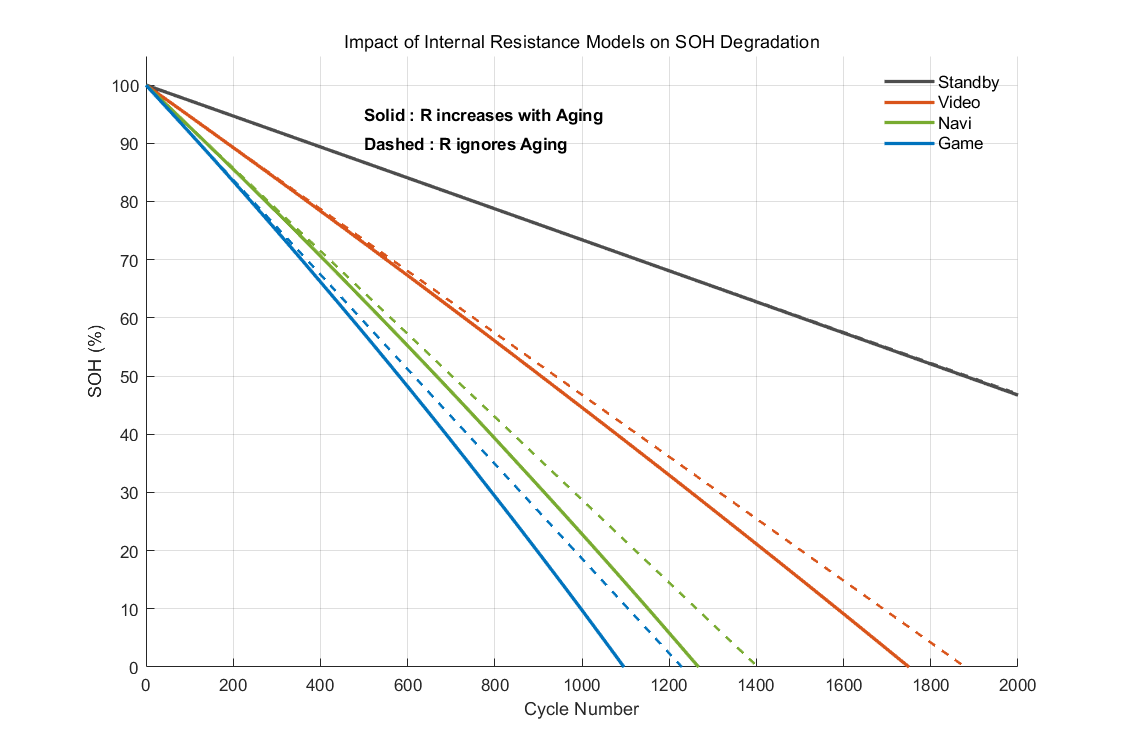
\includegraphics[width=0.6\textwidth]{figures/image_p2.png}
  \caption{SOH Degradation Curves under Different Internal Resistance Models}
  \label{fig:fig_internal_resistance}
\end{figure}

From the overall trend, the hybrid model predicts a significantly faster SOH degradation rate than the simplified model.
This difference arises because the internal resistance in the hybrid model increases with the number of cycles,
leading to higher ohmic losses and heat generation, which in turn accelerates battery capacity decay.
In contrast, the simplified model assumes a constant internal resistance,
failing to capture the cumulative impact of increasing internal resistance during aging on SOH,
and thus tends to overestimate the actual battery lifespan.
Significant differences exist in the impact of different usage modes on SOH degradation.
The standby mode, due to its extremely low power load during standby, results in minimal internal battery heating and chemical reaction rates, exhibiting the slowest degradation rate, with SOH remaining at about 47% after 2000 cycles.
The gaming mode, due to the highest load power causing intensified internal resistance heating and rapid degradation of electrode materials, leads to the fastest SOH degradation.
The hybrid model predicts that its SOH drops to nearly 0\% at about 1100 cycles,
while the simplified model predicts a lifespan of about 1220 cycles.
The degradation curves for video playback and navigation modes lie between the two.
The hybrid model predicts a lifespan of about 1750 cycles for the video scenario,
and about 1250 cycles for the navigation scenario.
The prediction differences between the hybrid and simplified models in these three scenarios are about 100-200 cycles, and are particularly pronounced in the later stages of battery life (SOH < 50%).
This indicates that the significant increase in internal resistance with battery aging accentuates the acceleration of capacity degradation.





\section{Recommendations}
\subsection{Suggestions for User Usage}
\begin{itemize}
  \item When engaging in high-load scenarios such as gaming or navigation, the battery depletion rate can be 8-10 times that of standby mode.
Therefore, under high load conditions, continuous use should not exceed 1.5 hours, or periodic cooling breaks should be taken.
After 1 hour of high-load gaming, it is recommended to rest for more than 15 minutes,
allowing the battery temperature to return to ambient temperature, thereby extending usage time and battery life.
  \item In indoor environments, reducing screen brightness appropriately can extend battery life and slow down battery aging.
  \item Standby screen-on limit: If the screen needs to be kept on for a long time (such as a bedside clock or display mode), forcibly setting the brightness to 50% can extend the battery cycle life.
When the screen does not need to be kept on, try to turn it off.
  \item Avoid playing while charging, as the Joule heat generated during charging combined with the heat generated by high load causes the battery temperature to rise, accelerating battery aging.
\end{itemize}
\subsection{Suggestions for the OS}
\begin{itemize}
  \item Integrate our UKF-based battery state estimation and time prediction model to inform users about battery status and remaining time.
  \item When high battery temperature is detected, throttle the CPU to limit power and reduce temperature, thereby slowing battery aging.
  \item Automatically adjust screen brightness based on ambient light to extend battery life.
\end{itemize}


\section{Model Evaluation and Further Discussion}
\subsection{Strengths}
\begin{itemize}
\item A second-order $RC$ equivalent circuit model is adopted, offering stronger physical interpretability than purely empirical fitting while enabling accurate and efficient SOC estimation.
\item A coupled thermodynamic model incorporating internal resistance and available capacity is introduced, capturing the dynamic impact of temperature on battery behavior and improving model consistency under complex operating conditions.
\item A genetic algorithm (GA) is employed for global parameter identification, reducing the risk of local optima and improving the robustness of key parameters ($R_0,R_1,R_2,C_1,C_2$) and initial SOC estimation.
\item The UKF effectively handles the nonlinear $E(SOC)$ observation, achieves fast-converging online SOC estimation, and provides confidence intervals to jointly assess prediction accuracy and reliability.
\end{itemize}

\subsection{Weaknesses}
\begin{itemize}
\item The power load model is simplified; real smartphone power consumption may exhibit stronger nonlinearity and abrupt variations due to complex interactions among hardware and software components.
\item Model performance depends on measured data for OCV fitting, parameter identification, and UKF noise settings ($Q_k$, $R_k$), requiring recalibration when battery conditions or system configurations change.
\item Using terminal voltage alone as the observation leads to limited information under low-dynamics conditions (e.g., standby), increasing uncertainty accumulation; moreover, UKF performance is sensitive to the choice of $Q_k$ and $R_k$.
\end{itemize}
\section{Conclusion}
This paper establishes a set of continuous-time models to characterize the nonlinear dynamic behavior of lithium batteries in smartphones, enabling power prediction and remaining time estimation. Based on a second-order RC equivalent circuit, a state-space differential model is derived using Kirchhoff’s laws to capture ohmic, electrochemical, and concentration polarization effects. A genetic algorithm (GA) is employed to identify key parameters, including internal resistances, polarization parameters, and initial SOC, by minimizing the terminal voltage RMSE.

The model is further extended to incorporate electro-thermal coupling, where Arrhenius-type relations describe the temperature dependence of resistance, available capacity, and battery aging (SOH). Finally, an unscented Kalman filter (UKF) is applied to estimate SOC and driving range, leveraging the sigma-point transformation to handle the nonlinear OCV–SOC relationship and obtain robust state predictions.
\newpage
\addcontentsline{toc}{section}{Reference}

\bibliographystyle{plain}   % 选用样式（plain / IEEEtran / elsarticle-harv ...）
\bibliography{reference}  
% \appendix
% \newpage
% \addcontentsline{toc}{section}{Report on Use of AI}
% \section*{Report on Use of AI}

% \subsection*{Gemini}

% \textbf{Query1:}

% 我现在要解决这个问题，需要查阅文献，为了很好解决这个问题，我应该查找哪些期刊，输入什么关键词?

% \textbf{Output1:}

% 这对于2026 MCM Problem A而言是一个非常关键的起步阶段。题目明确要求建立一个基于物理或机械推理的连续时间数学模型（Continuous-Time Model），并明确禁止仅使用离散曲线拟合或黑箱机器学习。为了满足这些硬性要求，本文重点查阅了结合电化学、电池物理与计算机系统功耗的文献。在期刊选择方面，本文重点关注两类文献：一类关注电池本身的物理特性（内部视角），另一类关注智能手机硬件对电量的消耗（外部负载视角）。电池物理与能源类期刊侧重电池内部机理和SOC估算，这类期刊提供了描述电压、电流、温度与剩余电量之间关系的微分方程，包括Journal of Power Sources（极高价值，涵盖锂离子电池的各类物理模型）、IEEE Transactions on Energy Conversion、Applied Energy、Electrochimica Acta以及IEEE Transactions on Industrial Electronics（常有SOC估算和等效电路模型的论文）。移动计算与系统类期刊侧重手机各部件功耗模型，这类期刊提供了量化屏幕、CPU、网络如何作为"负载"从电池中抽取电流的方法，包括IEEE Transactions on Mobile Computing（重点关注）、ACM Transactions on Embedded Computing Systems、Proceedings of MobiSys/MobiCom（虽然是会议，但包含大量关于智能手机能耗分析的顶会论文）以及IEEE Internet of Things Journal。

% 在高效检索关键词方面，建议将关键词组合使用（例如：Model A + Variable B）。针对连续时间模型要求的核心建模关键词，用于检索连续方程相关的微分方程框架，包括Lithium-ion battery Equivalent Circuit Model (ECM)（等效电路模型，最常用的连续时间模型基础）、Kinetic Battery Model (KiBaM)（动力电池模型，适合描述电量恢复效应）、State of Charge (SOC) estimation algorithm、Peukert's Law lithium-ion、Shepherd battery model（经典的放电电压方程）以及Electrochemical model single particle（单粒子模型，更物理但数学更复杂）。针对多因素影响的手机组件功耗关键词，用于将屏幕、CPU等转化为电流$I(t)$的函数，包括Smartphone power consumption profiling、OLED display power modeling brightness（屏幕亮度和功耗的函数关系）、DVFS (Dynamic Voltage and Frequency Scaling) power model（处理器负载与功耗的关系）、Cellular vs WiFi power tail energy（网络传输的尾部能量消耗模型）以及Background process energy drain Android/iOS。针对题目特定要求的环境与老化关键词，用于解决温度和老化/循环历史问题，包括Arrhenius equation battery degradation（用于描述温度对反应速率的影响）、Battery capacity fade modeling（容量衰减模型）、Lithium-ion low temperature performance以及Cycle life aging model。

% \textbf{Query2:}

% 手机锂电池的数据库应该怎么寻找，你能帮我找到符合这题的数据库吗?

% \textbf{Output2:}

% 由于手机电池（通常是软包电池）和通用的18650电池在化学特性上相似，学术界常用的数据集可以作为很好的起步。NASA Prognostics Center of Excellence (PCoE)是电池老化研究领域的"黄金标准"数据集，内容包含18650电池在不同温度、负载下的老化数据，其特点是数据非常详细，包含电压、电流、温度、阻抗谱(EIS)等，虽然主要是18650电池，但对算法验证完全通用，推荐使用Battery Aging Data Set，获取地址为NASA PCoE Data Repository。CALCE（马里兰大学）是另一个非常经典的数据库，被数千篇论文引用，其内容涵盖了多种正极材料（LCO, NCM, LFP）的电池，特点是包含了长时间的日历老化（Calendar Aging）和循环老化数据，非常适合研究电池的长期衰减，获取地址为CALCE Battery Group。Oxford Battery Degradation Dataset（牛津大学）的内容专注于长期电池退化，特点是测量非常精细，包含map-based的老化测试，特别适合建立高精度的电化学或等效电路模型，获取地址为Oxford Battery Intelligence Lab。Toyota/Stanford/MIT (Nature Energy Dataset)是一个针对快充和寿命预测的大规模数据集，内容包括124个磷酸铁锂/石墨电池的循环数据，特点是数据量非常大，专门用于训练机器学习模型来预测电池寿命(RUL)，如果想做AI模型，这个数据集是极佳的选择，获取地址为Stanford Pnas/Nature Energy Data。

% \textbf{Query3:}

% 我现在要查一下手机各模块的功率，请你给我推荐一些数据集，并且表明准确出处和链接

% \textbf{Output3:}

% 要准确查询手机各模块（CPU、GPU、屏幕、WiFi、GPS等）的功率，需要理解两类数据来源：开发者定义的"静态标准值"（最准确的参考标准）和用户行为的"动态数据集"。Android官方电源配置文件是最权威的模块参考值来源，如果想查找"某个模块的额定功耗是多少毫安"，这是最直接的来源，所有Android手机厂商在出厂时必须在系统文件中定义各个模块的电流消耗值，系统据此来计算"设置-电池"里的耗电百分比，数据内容包含CPU（不同频率下的电流）、WiFi（扫描/传输/空闲）、蓝牙、GPS、屏幕（开启/全亮）、音频DSP、摄像头等的具体电流值(mA)，适用场景为硬件功耗建模、查找特定模块的基准功耗，官方文档说明可见Android Open Source Project - Power Values，核心数据文件(XML)示例可见Google Git - power\_profile.xml，在该XML链接中可以看到诸如\texttt{<item name="wifi.active">200</item>}的代码，这意味着该参考设备WiFi活跃时消耗约200mA，不同厂商（小米、三星等）的该文件值不同，但结构一致。GreenHub Project是最大的真实设备电池数据集，这是一个学术界广泛使用的众包数据集，收集了全球数百万台Android设备的电池老化和耗电数据，数据内容包含电池电压、温度、充电/放电速率以及关联的硬件状态（屏幕是否开启、WiFi信号强度等），虽然主要是"整机功耗"，但可以通过数据分析拆解出各模块的影响，适用场景为真实环境下的功耗分析、电池老化研究、机器学习功耗预测，项目主页为GreenHub Project，数据集可在Hugging Face或Zenodo下载，也可以在Hugging Face上搜索GreenHub相关数据集，或者直接通过他们的Datasets页面申请访问，相关论文为GreenHub: A Large-Scale Collaborative Dataset to Battery Consumption Analysis of Android Devices (IEEE Access, 2021)。Kaggle移动设备与传感器数据集适合快速上手，Kaggle上有许多经过清洗的针对性数据集，虽然不如AOSP底层，但适合做数据分析练手，推荐数据集为"Smartphone Energy Consumption Dataset"或"Mobile Device Usage Dataset"，数据内容通常包含App使用时长、屏幕开启时长、数据流量消耗与剩余电量的对应关系，相关链接包括Mobile Device Usage and User Behavior Dataset (Kaggle)以及Smart Home Energy Consumption (Kaggle)（注：此类数据集有时混杂智能家居，需筛选Mobile标签）。学术级数据集CRAWDAD是一个无线网络和移动计算的数据集存档，非常硬核，数据内容包含极其精细的WiFi信号追踪、蓝牙交互和移动能耗日志，出处链接为CRAWDAD (Community Resource for Archiving Wireless Data At Dartmouth)，可在站内搜索"Power"或"Battery"。如果需要"绝对数值"（例如WiFi芯片到底消耗多少功率），不要找CSV数据集，应直接查看AOSP的power\_profile.xml，功率(mW)的计算公式为电流(mA，从xml获取)乘以电压(V，通常为3.8V或4.2V)，例如XML中gps.on为50mA，电压3.8V，则GPS功率约为190mW。如果需要"行为数据"（例如屏幕亮度和耗电量的线性关系），应使用GreenHub的数据。


\end{document}
\